\chapter{Dynamics of the gene expression machinery during an acetate-glucose upshift}
\chaptermark{Gene expr. machinery during an upshift}
\label{chap:experiments}

%\textit{"If reality does not fit the concept, too bad for reality."} -- Georg Wilhelm Friedrich Hegel

\selectlanguage{french}
\section*{Résumé en français du Chapître \thechapter : Dynamique de la machinerie d'expression génique lors d'une transition acétate vers glucose.}

Résumé d'environ 6-8 paragraphes (2 pages).
\selectlanguage{english}

\section{Introduction}

Most studies of the growth of microorganisms have been done at steady state.
This is a reasonable and logical choice given that at steady state, the behavior of microorganisms is reproducible, which helps uncovering simple theories to apprehend their inherent complexity.
But while this condition can be easily achieved in the laboratory, microorganisms naturally spend very little time in steady state.
This motivated the construction of a new theoretical framework in Chapter~\ref{chap:theory} to study growth laws during growth transitions.

The principles underlying regulatory processes in dynamical conditions appear to be different from those applying at steady state.
We showed that regulatory strategies approaching the theoretical optimal, given by bang-bang control of gene expression machinery, have to be able to effect abrupt and strong variations in the activity of a gene.
It was seen that for implementing such strategies the regulatory system needs to be capable of sensing the internal state of the cell and not just the environment.
A near-optimal transition also requires information of several different variables, whereas for maintaining a steady state with maximal biomass accumulation a single variable turned out to be sufficient in our theoretical framework.
Interestingly, we showed that the ppGpp regulatory system of \textit{E. coli} fulfills the requirement of such a regulatory strategy, by implementing an on-off strategy for regulating the synthesis of ribosomes.
However, although this provides circumstantial evidence that bacteria control resource allocation in a manner consistent with theoretical optimality, experimental data are necessary to decide if an on-off strategy is at work in \textit{E. coli} during growth transitions.

Unfortunately, far more information is available on ribosome abundance at steady state than during growth transitions~\cite{scott_interdependence_2010,gausing_regulation_1980}.
The main reason for this bias on steady-state conditions is that, from an experimental point of view, growth transitions are hard to control and may depend on the history of the culture~\cite{ng_damage_1962,dufrenne_effect_1997,shaw_effect_1967,mcmeekin_predictive_2002,cheroutre-vialette_application_2002}.
However, as we discussed in Section~\ref{sec:discussion}, the few studies that have been reported seem to be consistent with our predictions, in the sense that they indicate that during growth transitions, the synthesis rate of ribomoses oscillates~\cite{gausing_regulation_1980,zengel_transcription_1986} and the ppGpp concentration manifests a rapid succession of increases and decreases~\cite{friesen_synthesis_1975,murray_control_2003}.
But we cannot decisively validate or disprove the model predictions from measurements that were carried out at the population level, where it is inherently hard to identify switching patterns.
What is needed for the verification of our predictions are dynamical single-cell measurements of the ribosome concentration during well-controlled growth transitions.
While the observation of an on-off strategy would show that simple models of the type introduced in Chapter~\ref{chap:theory} are instrumental in gaining a better understanding of microbial physiology, its refutation would also raise interesting questions. 
If maximization of growth rate and biomass accumulation have been retained by natural selection in \textit{E. coli}, which factors would prevent the cell from behaving optimally from a theoretical point of view?

The aim of this chapter is to measure \textit{in vivo}, during a growth transition, the resource allocation profile $\alpha (\cdot)$ and compare its dynamics with the gold standard established in Chapter~\ref{chap:theory}.
To this end, we have measured ribosomal abundance of \textit{E. coli} at the single-cell level during a nutrient upshift.
More precisely, we constructed a strain in which a fluorescent marker has been attached to a ribosomal subunit, thus allowing the \textit{in-vivo} monitoring of (changes in) the abundance of ribosomes.
In collaboration with Irina Mihalcescu of the Laboratoire Interdisciplinaire de Physique, we cultivated this \textit{E. coli} strain in a microfluidic device, allowing the long-term imaging of individual cells in well-controlled conditions, notably involving a classic upshift experiment from growth in minimal medium with acetate to minimal medium with glucose.
We then developed a Kalman smoothing method, in collaboration with Eugenio Cinquemani of Inria Grenoble -- Rh\^{o}ne-Alpes, to reconstruct $\alpha (\cdot)$  from the estimates of the variations of the growth rate and the relative ribosomal synthesis rate.
While the preliminary results presented here do not allow a decisive validation of the expected behavior, among other things due to the difficulties that were encountered during the experiments and the image analysis, we believe they are promising as a first step towards the better understanding of global resource allocation during growth transitions.

For clarity, the model of resource allocation during growth transitions developed in Chapter~\ref{chap:theory} is reproduced here, where dotted variables represent time derivatives:
\begin{eqnarray}
\dot{p}(t) &=& e_M(t)\cdot (1/\beta - r(t)) - \frac{k_R \cdot p(t)}{K_R + p(t)}\cdot r(t) \, (1+\beta\, p(t)), \label{eq:pdef-exp}\\
\dot{r}(t) &=& \frac{k_R \cdot p(t)}{K_R + p(t)}\cdot r(t) \, (\alpha(t) - \beta\, r(t)). \label{eq:rdef-exp}
\end{eqnarray}
In this form, it contains 4 variables ($e_M(t)$, $p(t)$, $r(t)$, $\alpha (t)$) and 3 parameters ($\beta$, $k_R$, $K_R$).
$e_M(t)$ [min\textsuperscript{-1}] is an indicator of the richness of the environment.
$p(t)$ [g.L\textsuperscript{-1}] is the precursor concentration inside the cell.
$r(t)$ [g.L\textsuperscript{-1}] is the concentration of gene expression machinery inside the cell.
$\alpha (t)$ [$\emptyset$] is the fraction of resources allocated to the synthesis of gene expression machinery.
$k_R$ [min\textsuperscript{-1}] is the rate constant of macromolecular synthesis.
$K_R$ [g.L\textsuperscript{-1}] is the half-saturation constant of macromolecular synthesis.
$\beta$ [L.g\textsuperscript{-1}] is the inverse of the cellular density of macromolecules, assumed to be constant.



\section{Results}

\subsection{Experimental design}
\label{sec:exp_design}

How can one measure the resource allocation variable in \textit{E. coli} cells?
There is no direct way to quantify $\alpha (\cdot)$ in an experiment, mostly because of its abstract nature.
To correctly reconstruct it, one has to know the value of every single term in the equations in which it appears.
In the model of Eqs~\ref{eq:pdef-exp}-\ref{eq:rdef-exp}, $\alpha$ only appears in Eq.~\ref{eq:rdef-exp}.
We can therefore identify $\alpha (t_k)$ for each time $t_k$ when the terms $\beta r(t_k)$, $\dot{r}(t_k)$, and $\frac{k_R \cdot p(t_k)}{K_R + p(t_k)} \cdot r(t_k)$ are known, or equivalently, the six individual components $r(t_k)$, $\dot{r}(t_k)$, $p(t_k)$, $k_R$, $K_R$, $\beta$ they are composed of.
Even when assuming that the parameters $k_R$, $K_R$, and $\beta$ are known, or at least easy to estimate independently, reconstructing the dynamics of $\alpha$ would require estimation of the (changes in) concentration of the gene expression machinery ($r$, $\dot{r}$) and the precursor concentration $p$.

Are such measurements feasible in practice?
The abundance of ribosomes can be quantified, for instance, by measuring the total RNA of the cell~\cite{scott_interdependence_2010}, or using radioactive markers \cite{gausing_regulation_1980,zengel_transcription_1986}, fluorescent labels~\cite{bakshi_superresolution_2012}, or mass spectrometry techniques~\cite{hui_quantitative_2015}.
However, only the use of fluorescent proteins complies with our need for real-time single-cell quantification.
Obtaining an estimate of precursor abundance is even more challenging, since there is no clear proxy for the totality of precursors in the cell and, while absolute quantification of all internal metabolites has been achieved in \textit{E. coli}~\cite{bennett_absolute_2009}, this method is also not suitable for a dynamical estimation in individual cells.

The problem of quantifying $\alpha (\cdot)$ can be simplified by applying a transformation of the model of Eqs~\ref{eq:pdef-exp}-\ref{eq:rdef-exp}.
Taking into account that by construction the growth rate $\mu(t)$ is given by
\[
	\mu (t) = \beta \frac{k_R \cdot p(t)}{K_R + p(t)} \cdot r(t),
\]
we can rewrite Eq.~\ref{eq:rdef-exp} as follows
\begin{equation}
\label{eq:dot_r}
\dot{r}(t) = \mu (t) \, \left(\frac{\alpha(t)}{\beta} - r(t) \right).
\end{equation}
The problem of estimating $\alpha(\cdot)$ is thus equivalent to the problem of estimating $r(\cdot)$, $\dot{r}(\cdot)$, $\mu (\cdot)$ and $\beta$.
If we are satisfied with estimating $\alpha$ up to a constant factor $\beta$, dynamically measuring the ribosome concentration and the growth rate would make $\alpha (\cdot) / \beta$ identifiable. 

Given that fluorescent reporters of ribosomal proteins can provide information on both $r(\cdot)$ and $\dot{r}(\cdot)$ \cite{zulkower_robust_2015}, the above reformulation of the problem is promising for the purposes of our study.
Moreover, since the predicted bang-bang profiles in gene activity are easily hidden at the population level if cells are not synchronous, which is generally the case, expression of the ribosomal genes need to be monitored at high sampling density on the single-cell level, which is also possible with fluorescent reporters.
Inspired by previous work~\cite{bakshi_superresolution_2012}, we therefore constructed an \textit{E. coli} strain in which the S2 ribosomal subunit, encoded by the gene \textit{rpsB}, has been tagged with a green fluorescent protein (GFP).
The strain with the chromosomal \textit{rpsB-gfp} fusion produces fluorescent ribosomes that are quantifiable \textit{in vivo} in single cells while not affecting the growth rate (see Material and Methods~\ref{sec:methods_strain} and~\cite{bakshi_superresolution_2012}).
Monitoring single cells of this strain, by time-lapse fluorescence microscopy, thus makes it possible to estimate $r(\cdot)$ and $\dot{r}(\cdot)$ and reconstruct $\mu(\cdot)$.

The growth conditions also need to be carefully chosen for this study.
In natural environments, for many bacteria one of the most frequently encountered growth transitions, or at least the transition on which selection is expected to operate, is the transition from stationary phase in a nutrient-deprived medium~\cite{gefen_direct_2014} to (exponential) growth after the renewed availability of nutrients.
The transition from stationary to exponential phase is difficult to study though as many hard-to-control parameters play a role, including the duration of the nutrient stress, the composition of the medium before growth arrest, and the accumulation of waste products in the medium~\cite{ehrenberg_mediumdependent_2012}.
As a consequence, growth resumption only occurs after a lag phase of variable duration~\cite{ng_damage_1962,dufrenne_effect_1997,shaw_effect_1967,mcmeekin_predictive_2002,cheroutre-vialette_application_2002}, which is not included in the model.
For this reason, we decided to focus on a transition from exponential growth on a poor carbon source (acetate) to exponential growth on a rich carbon source (glucose) in a well-defined minimal medium.
By construction, this steady-state-to-steady-state transition requires a long acquisition time before and after the shift, respectively, to ensure that the cells have no memory of their physiological state before the transition and have enough time to reach the new steady state after the transition.
The use of the mother machine, a microfluidic device that was designed to sustain exponential growth for long periods of time, is therefore a good choice for this purpose.
It allows to maintain a constant flow of fresh medium and to effect fast transitions by switching the medium (see Material and Methods~\ref{sec:growth_condition} and \ref{sec:microflu}).
The complete experimental plan is summarized in Fig.~\ref{fig:experiment_schema}.

\begin{figure}[tb]
\centering
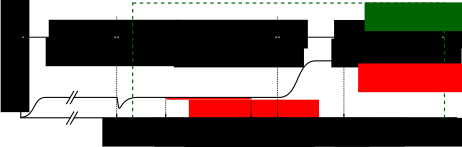
\includegraphics[scale=1]{./Fig/experiment_schema}
\caption{
\textbf{Schematic outline of the upshift experiment.}
The goal is to measure the fluorescence and length/area of \textit{E. coli} \textit{rpsB-gfp} cells during an acetate-to-glucose upshift.
We use M9 minimal medium supplemented with 0.2\% of acetate or glucose (see Material and Methods~\ref{sec:growth_condition}).
A preculture was started from glycerol stock for 2.5 days on 0.2\% acetate in batch condition (shake flask).
The day of the experiment, the cells were injected into the mothermachine and fed by a constant flow of fresh 0.2\% acetate medium (see Material and Methods~\ref{sec:microflu}).
Fluorescence and phase contrast images were taken every 5 minutes.
After 20~h, the feeding media was switched to 0.2\% glucose and maintained for 20~h while continuing image acquisition.
Time 0 corresponds to the moment of the acetate-glucose upshift.
}
\label{fig:experiment_schema}
\end{figure}

\subsection{Data acquisition}
\label{sec:data_acquisition}

An experiment following the plan of Fig.~\ref{fig:experiment_schema} was carried out, over a period of 40~h, but encountered a number of difficulties.
First, the motor displacing the microscope along the Z-axis intermittently stalled, thus deactivating the autofocus and the Z-compensation for the tilt of the microfluidic device in the XY plane.
As a consequence, until the experimenter manually intervened, many of the images acquired were out of focus.
This is the reason why data points between -720 and -150 min are not exploitable, but fortunately the experiment was planned in such a way that when it really mattered, notably around the growth transition, someone was present to monitor the microscope.
Second, at around 7~h after the nutrient upshift, the bacteria started to die for reasons that are unknown, the most plausible hypothesis being a phage contamination (see Discussion~\ref{sec:chap3_discussion}).
Data analysis was therefore limited to 550 min after the upshift, when roughly 3/4 of the cells were still growing.
For these and other reasons (see Section~\ref{sec:chap3_discussion}), the experiment will have to be repeated, but there was no time left for this in the framework of my PhD thesis.

The acquired data consisted of phase contrast and fluorescence images of 60 wells in total, in four different fields.
While quite a few image analysis programs have been reported in the literature~\cite{klein_tlm-tracker:_2012,wang_image_2010,young_measuring_2012,paintdakhi_oufti:_2016}, and some of these specifically address the mother machine design of the microfluidic device~\cite{wang_robust_2010,sachs_image-based_2016}, they all presented limitations when applied to our data.
For instance, the segmentation algorithms experienced difficulties due to the low resolution of the camera, and the phase contrast images had a superposed reflection band due to the microfluidic device.
Moreover, the fluorescence density was concentrated in hot spots (Fig.~\ref{fig:data_acquisition}) and its intensity varied during the experiment. 
While this was expected, since ribosomes are localized in the cell poles~\cite{bakshi_superresolution_2012} and ribosomal abundance is known to vary with the growth rate~\cite{scott_interdependence_2010}, it complicated automatic segmentation on the fluorescence images.

For these reasons, the image analysis carried out for this chapter has been much simplified. 
First, we have focused on the cell at the bottom of each well, since this avoids the tracking of individual cells across several generations and ensures that the descendance of this cell can be followed throughout the experiment.
Second, segmentation was done by manually selecting two pixels, one at each pole of the cell.
These pixels were used to create a rectangle surrounding the cell (Fig.~\ref{fig:data_acquisition} and Material and Methods~\ref{sec:cell_segmentation}).
After background correction (Material and Methods~\ref{sec:cell_segmentation}), the fluorescence intensity in units RFU was evaluated for each pixel in the rectangle, as well as the length of the cell, defined by the distance in pixels between the poles (Fig.~\ref{fig:data_acquisition}).
The fluorescence density for the entire cell [RFU/pixel/cell] was computed by dividing the sum of the fluorescence intensities of the pixels in the rectangle by the total number of pixels in the rectangle.
Although we are well aware that the above procedure can be improved on many counts (Section~\ref{sec:chap3_discussion}), we nevertheless believe that it provides a reasonable approximation of the quantities of interest and a valid starting-point for the estimation of the growth rate and the resource allocation profile in the remainder of this chapter.   


\begin{figure}[p]
\centering
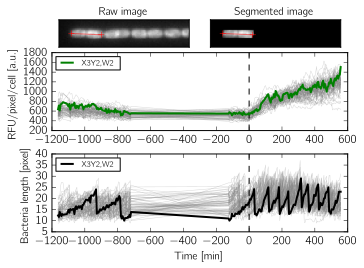
\includegraphics[scale=1]{./Fig/data_acquisition}
\caption{
\textbf{Results of data acquisition.}
We imaged 6 fields (X[1-3]Y[1-2]) each containing 15 wells (W[0-14]) for $\sim$40~h.
From the 90 wells, 68 were suitable for further analysis (the others being empty, out of frame for some period of time, or plugged).
For all wells, data points are missing in the interval between [-720,-150] because the camera was out of focus.
We stopped the analysis at 550~min, when about 3/4 of the bacteria were still growing, before the entire population died within a few hours for an unknown reason.
The image labeled "Raw image" is the last image analyzed for the highlighted well.
The bacterium on the left of this image was manually segmented by selecting two pixels at the poles on the fluorescence images (red cross).
A 6-pixel-wide rectangular mask was computed for each image, resulting in the "Segmented image" on the right.
Fluorescence intensities are expressed in Relative Fluorescence Units (RFU) on a 16-bit image and were corrected for camera background, but not autofluorescence background (Material and Methods~\ref{sec:cell_segmentation} and Discussion~\ref{sec:chap3_discussion}).
The fluorescence intensity of the cell, expressed in units RFU/pixel/cell, was computed by dividing the sum of the fluorescence intensities of the pixels in the rectangle by the total number of pixels in the rectangle.
The cell length is the distance in pixels between the two poles (red line).
The thick lines in green and black highlight the time-varying length and fluorescence density for the cell visible in the top images, labeled "X3Y2, W2".
The vertical dashed lines represent the time of the upshift from growth on acetate to growth on glucose.
}
\label{fig:data_acquisition}
\end{figure}

In total, we obtained time courses of fluorescence density [RFU/pixel/cell] and the length for 68 bacterial cells (Fig.~\ref{fig:data_acquisition}).
The fluorescence density appears constant during growth on acetate (before time 0) and immediately increases when the carbon source is switched to glucose.
Inspection of the cellular length shows that the division frequency abruptly increases after the nutrient upshift, corresponding to a higher growth rate.
Unfortunately, while steady-state growth on acetate was reached before the upshift, the fluorescence density profile suggests that the experiment did not continue long enough to ensure that a new steady state on glucose was reached.
However, the data before and after the nutrient upshift are exploitable.
What do we observe if we estimate the growth rate and the resource allocation profile from these data?

\subsection{Data analysis using Kalman smoothing}
\label{sec:res_kalman}

As we presented in section~\ref{sec:exp_design}, our goal is to reconstruct the signal $\alpha (\cdot)$ during a growth transition.
By modeling \textit{E. coli} as a cylinder, the volume can be assumed directly proportional to the length of the cell.
If we assume a negligible background of autofluorescence (see Material and Methods~\ref{sec:cell_segmentation}), the fluorescence concentration in the cell can be assumed proportional to the ribosome concentration.
More precisely, based on the available data, we have the following measurement model at each time-point $t_k$, $0\leq k \leq N-1$:
\begin{eqnarray}
L(t_k) &= \lambda \cdot V(t_k) + \epsilon_k, \label{eq:mes_L}\\
F(t_k) &= \gamma \cdot r(t_k) + \eta_k, \label{eq:mes_F}
\end{eqnarray}
where $L(t_k)$ and $F(t_k)$ are the length and fluorescence density in units RFU/pixel measured at time $t_k$, respectively,  and $V(t_k)$  and $r(t_k)$ the corresponding actual volume and ribosome concentration at time $t_k$, respectively. ($\lambda$,$\gamma$) are unknown proportionality constants, and ($\epsilon_k$,$\eta_k$) uncorrelated sequence of measurement noise assumed normally distributed with mean 0.

As explained in Section~\ref{sec:exp_design}, reconstructing $\alpha (\cdot)$ requires information on $\mu (\cdot)$, $r(\cdot)$ and $\dot{r}(\cdot)$.
From Eq.~\ref{eq:mes_F}, we can obtain $r(\cdot)$ and $\dot{r}(\cdot)$ by smoothing interpolation and differentiation.
Similarly, $\mu (\cdot)$ can be derived from Eq.~\ref{eq:mes_L} as it is defined by
\[
\dot{V}(t) = \mu (t) \cdot V(t).
\]
However, smoothing interpolation is particularly sensible to the boundary conditions.
Since each division in the time series generates a new boundary condition, smoothing interpolation of our data is expected to be little robust.
For this reason, the growth rate of single cells is usually estimated by fitting an exponential function to the volume data between each cell~\cite{wang_robust_2010,izard_synthetic_2015}.
While this is suitable when bacteria are at steady state, it is not applicable during a growth transition, where we expect the growth rate to vary between successive divisions.
Other techniques are less sensible to the above problem~\cite{zulkower_robust_2015}, and we decided to use Kalman smoothing for our purpose~\cite{kailath_linear_2000,jazwinski_stochastic_2007}.

Kalman filtering~\cite{kalman_new_1960} is a Bayesian algorithm using a series of noisy measurements to predict the state of a dynamical system.
It has been extensively used in engineering applications (guidance, tracking, control, ...) requiring the real-time estimation of hidden variables in a dynamical system from present and past measurements.
Kalman smoothing is an extension of Kalman filtering using information about past and present but also future measurements of the state of the system, and is widely applied to estimate unknown inputs in time series analysis~\cite{kailath_linear_2000,jazwinski_stochastic_2007}.
The advantage of Kalman filtering with respect to Kalman smoothing is that it uses all available information to estimate the hidden variables of a dynamical system, in applications where a real-time response is not required.
For our problem, at each time step $t_k$, our hidden variables are the resource allocation variable $\alpha (t_k)$ and the growth rate $\mu (t_k)$, while the available information consists of the $N$ measurements $\left\{ F(t_0), F(t_1), ..., F(t_{N-1}) \right\}$ and $\left\{L(t_0), L(t_1), ..., L(t_{N-1}) \right\}$ that were taken during the experiment.

The Kalman filtering problem can now be formulated as follows.
The state of a growing bacterial cell is described by the dynamical system
\begin{eqnarray}
\dot{r}(t) &=& \mu (t) \cdot \frac{\alpha(t)}{\beta} - \mu (t) \cdot r(t),\\
\dot{V}(t) &=& \mu (t) \cdot V(t),
\end{eqnarray}
with initial conditions $r(0) = r_0$, $V(0) = V_0$, and the following measurement model:
\begin{eqnarray}
L(t_k) &= \lambda \cdot V(t_k) + \epsilon_k,\\
F(t_k) &= \gamma \cdot r(t_k) + \eta_k,
\end{eqnarray}
where the variables are as defined as for Eqs~\ref{eq:dot_r}, \ref{eq:mes_L} and \ref{eq:mes_F}.
While $\beta$ can be obtained from the literature (Chapter~\ref{chap:theory}), $\lambda$ and $\gamma$ are unknown parameters that need to be estimated along with $\alpha (\cdot)$ and $\mu (\cdot)$.
Since we are satisfied with a qualitative reconstruction of $\alpha (\cdot)$, we can simplify the system by defining $r_\gamma = \gamma \cdot r$ and $V_\lambda = \lambda \cdot V$.
The dynamical system is consequently rewritten as
\begin{eqnarray}
\dot{r}_\gamma(t) &=& \mu (t) \cdot\frac{\gamma \cdot \alpha(t)}{\beta} - \mu (t) \cdot r_\gamma (t),\label{eq:r_prob}\\
\dot{V}_\lambda (t) &=& \mu (t) \cdot V_\lambda (t),\label{eq:V_prob}
\end{eqnarray}
with initial conditions $r_\gamma (0) = \gamma r_0$, $V_\lambda (0) = \lambda V_0$, and the new measurement model:
\begin{eqnarray}
F(t_k) &= r_\gamma (t_k) + \eta_k,\label{eq:F_prob}\\
L(t_k) &= V_\lambda(t_k) + \epsilon_k.\label{eq:L_prob}
\end{eqnarray}
The Kalman filtering problem thus becomes the reconstruction of $\gamma \alpha (\cdot) / \beta$ and $\mu (\cdot)$ from measurements $\left\{ F(t_0), ..., F(t_{N-1}) \right\}$ and $\left\{L(t_0), ..., L(t_{N-1}) \right\}$.

Note that the above problem is not linear, whereas Kalman filtering was initially introduced for linear systems~\cite{kalman_new_1960,kailath_linear_2000}.
For this reason, we use a nonlinear extension of Kalman smoothing called unscented Kalman smoothing~\cite{julier_new_1997,jazwinski_stochastic_2007}.
Details about its exact implementation are available in Material and Methods~\ref{sec:meth_kalman}.
While it is feasible to simultaneously reconstruct the signals $\mu (\cdot)$ and $\gamma \alpha (\cdot) / \beta$ using Kalman smoothing, it is not necessary in our case and might lead to unstable results.
We therefore decided to proceed in two steps: first reconstruct $\mu(\cdot)$ from the measurements $L(\cdot)$, than inject this result into the reconstruction of $\gamma \alpha(\cdot) / \beta$ from the measurements $F(\cdot)$.

\subsection{Estimation of growth rate and resource allocation profile}
\label{sec:estim_gr_ra}

\subsubsection*{Growth rate estimation}

As presented in the previous section, we want to reconstruct the growth rate $\mu$ defined by Eq.~\ref{eq:V_prob}, using measurements of the length $L$ defined by Eq.~\ref{eq:L_prob}.
Note that Kalman smoothing is a procedure that returns the expected mean and covariance of the state of a dynamical system, given the  measurements.
Therefore, reconstructing $\mu$ requires it to be explicitly included as a state variable of the dynamical system.
This provides constraints on the variation of $\mu$ that have the effect of a regularization.
In particular, in the Kalman smoothing procedure, we model the variations of $\mu$ as the outcome of a stochastic process.
The laws describing this process play the role of a prior on the expected regularity of $\mu$ (the more noisy the process, the less constrained the variations of $\mu$).
In particular, we define $\mu$ as the double integral of a Gaussian white noise $w$:
\[
\dot{\mu} = v(t), \;\;\;\; \dot{v} = w(t),
\]
where $v$ is an intermediate variable and $w(t)$ is assumed normally distributed with mean 0 and standard deviation $\theta$: $w(t) \sim \mathcal{N}(0, \theta)$.
The resulting system then becomes
\begin{eqnarray}
\dot{V_\lambda}(t) &=& \mu (t) \cdot V_\lambda (t),\nonumber\\
\dot{\mu}(t) &=& v(t),\label{eq:full_mu_prob}\\
\dot{v}(t) &=& w(t),\nonumber
\end{eqnarray}
with the measurement model
\begin{equation}
L(t_k) = V_\lambda(t_k) + \epsilon_k,
\end{equation}
and the initial conditions
\[
V_\lambda (0) = V_{\lambda,0}, \;\;\;\; \mu (0) = \mu_0 , \;\;\;\; v(0) = v_0,
\]
that may themselves be Gaussian random variables with some given statistics.
The advantages of this regularization method are that the reconstructed $\mu$ is guaranteed to be second-order differentiable.
It is also equivalent to other methods like Tikhonov regularization~\cite{tikhonov1977solutions,tikhonov1963solution,de_nicolao_nonparametric_1997}, which minimizes least-square differences between predictions and observations along with penalizing the variations of the input.

Our prior is thus entirely contained in the parameters of the Kalman procedure:
\begin{itemize}
\item the mean of the initial state $(V_{\lambda,0}, \mu_0, v_0)$,
\item the covariance of the initial state $(V_{\lambda,0}, \mu_0, v_0)$,
\item the transition covariance for the derivatives of $V_\lambda$, $\mu$ and $v$ (see below),
\item the variance of the observation noise $\epsilon_k$.
\end{itemize}
The mean and covariance of the initial state $(V_{\lambda,0}, \mu_0, v_0)$ represent the knowledge we have of the initial values of the variables.
For instance, if we know exactly the initial value of the growth rate $\mu$ (\textit{via} independent measurements or literature data), we can use it as mean for $\mu_0$ along with a very small variance.
This will constraint the signal reconstruction by penalizing deviations from this value at $t=0$.
On the contrary, if we are very uncertain of the value for $V_{\lambda,0}$ (because cells are not synchronized, and can be in any state when the data acquisition starts), we can use a large variance for this initial condition.
In our framework, there is no transition covariance for $V_\lambda$ and $\mu$, because they are not the result of a stochastic process (the equations that define their derivatives are fully deterministic).
However, by definition $v$ is the result of a stochastic process of mean 0 and transition variance $\theta^2$.
This value is crucial and represents the intensity of the white noise $w$ that serves as prior for the regularization of $\mu$.
The smaller its value, the more the variations of $v$ are penalized, hence the smoother the reconstructed $\mu (\cdot)$.
Finally, the variance of the observation noise $\epsilon_k$ is simply the expected measurement noise.
Together, these parameters represents the \textit{prior} information we have on the initial conditions, the smoothness of the reconstructed signal, and the precision of our measurements, in order to reconstruct the growth rate $\mu (\cdot)$.
As we will see below, we widely use these properties to overcome the difficulties introduced by the discontinuities following cell divisions.

The observation of the length $L$ of growing bacterial cells is inherently discontinuous, due to the division of cells at regular time-points (Fig.~\ref{fig:data_acquisition}).
The estimation problem can therefore not be solved for the experiment as a whole, but only for the time-intervals between two successive division events, when the cell length is expected to change continuously.
We localize the division events by identifying the time points at which the empirical derivative of the length is below an arbitrary threshold, and correspondingly slice the total duration of the experiment into time-intervals with continuous changes of cell length.
The simplest way to proceed from there on would be to treat each portion independently.
However, by doing this we would lose important information, since the growth rates of a mother and its daughter cells are expected to be similar.
In other word, while not necessary continuous, the growth rate of new-born cells will depend strongly on the growth rate of their mother just before division.
This can be easily taken into account in the Kalman smoothing procedure by exploiting the prior information about the initial mean and covariance of the system variables.
In particular, we set the mean of the initial growth rate of a daughter cell equal to the final estimated growth rate of the mother cell, while defining a reasonable variance of the growth rate to allow for uncertainty.
The results of this Kalman smoothing procedure, along with the exact parameters used, are reported in Fig.~\ref{fig:growth_rate_estimation} and Material and Methods~\ref{sec:meth_kalman}.

\begin{figure}[p]
\centering
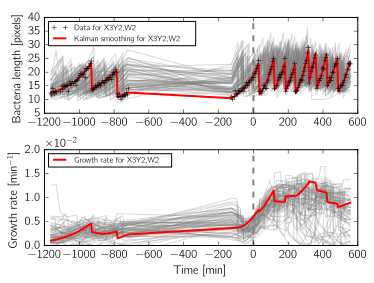
\includegraphics[scale=1]{./Fig/growth_rate_estimation}
\caption{
\textbf{Growth-rate estimation using Kalman smoothing based on measurement of the length of bacteria growing in a microfluidic device.}
Gray lines represent the estimation of the time-varying length (upper plot) and growth rate (lower plot) of 68 cells by the unscented Kalman smoothing procedure.
The solid red lines highlight the result for one particular cell, located at the bottom of the well labelled "X3Y2, W2", while black crosses in the top graph are the data points for this cell.
The vertical dashed lines represent the time of the upshift from growth on acetate to growth on glucose.
As prior for the algorithm, we used an observation variance of 9 pixels\textsuperscript{2} for the length $L$.
The transition variance $\theta^2$ (\textit{i.e.}, the smoothing factor for $\mu$) is fixed at $10^{-8}$~min\textsuperscript{-6}.
Inheritance between mother and daughter cells is taken into account by systematically choosing an initial mean growth rate equal to the last estimated value for $\mu$ before cell division, and to half the last estimated value for $V_\gamma$, bearing in mind that \textit{E. coli} cells divide symmetrically.
At the start of the experiment, when no mother cell is available to provide initial estimates, the above values were fixed at 15~pixels for $V_\gamma$ and 0.004~min\textsuperscript{-1} for $\mu$.
The variances associated with these means are 16~pixels\textsuperscript{2} and $10^{-4}$~min\textsuperscript{-2}, respectively for $V_\gamma$ and $\mu$.
The initial mean of $v$ is set equal to 0, with an initial variance of $10^{-8}$~min\textsuperscript{-6}.
All the cross-covariances are set to 0 because the system variables are independent by construction.
}
\label{fig:growth_rate_estimation}
\end{figure}

On average, the results presented in~Fig.~\ref{fig:growth_rate_estimation} show a roughly constant growth rate on acetate, followed by a quick increase after the upshift.
Contrary to what was visible in the plot with the fluorescence data, a steady state for the growth rate seems to have been reached before the end of the experiment.
When considering the individual cells, the results are more difficult to interpret.
A significant part of the cells stopped growing before the end of the experiment, probably due to the fact that all cells die from an unknown cause around the end of the experiment. 
As a consequence, the analysis has been limited to a time-interval after the upshift in which roughly 3/4 of the cells are still growing.
Interestingly, 1/6 of the cells exhibit growth rate oscillations, with a 1~h-long pause around 200 min after the upshift, followed by a recovery of the growth rate until the end of the experiment (see~\ref{S2_Figure}  and \ref{S3_Figure}).
In order to focus the analysis, we decided to classify the cells in three categories: dying cells (N=12) for which the growth rate drops to zero after the upshift, pausing cells (N=11) for which the growth rate drops to zero after the upshift and then recovers, and finally so-called normal cells (N=45) which do not exhibit any of the above behaviors (see~\ref{S2_Figure} and \ref{S3_Figure})
In what follows, we focus on the 45 normal cells (Fig.~\ref{fig:growth_rate_estimation_median}) which show a globally coherent behavior in the time window considered here.

\begin{figure}[tb]
\centering
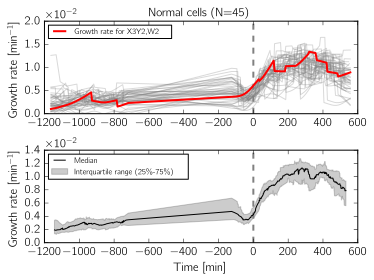
\includegraphics[scale=1]{./Fig/growth_rate_estimation_median}
\caption{
\textbf{Growth-rate estimation using Kalman smoothing for the normal cells only.}
The top graph is the same as the bottom graph of Fig.~\ref{fig:growth_rate_estimation}, except that the dying and pausing cells were removed.
The bottom graph shows the 25\% (lower gray curve), 50\% (solid black curve) and 75\% (upper gray curve) quartiles, computed at each time step.
The gray area represents the interquartile range.
}
\label{fig:growth_rate_estimation_median}
\end{figure}

\subsubsection*{Estimation of resource allocation profile}

In order to estimate the time-varying allocation of resources after the upshift, we use a similar Bayesian regularization approach as for the estimation of the growth rate.
We note $u(t) = \gamma \alpha (t) / \beta$ the resource allocation input that we wish to reconstruct.
With $\hat{\mu}$ the estimation of $\mu$ obtained in the previous section, the full model for the reconstruction of $u (\cdot)$ is given by
\begin{eqnarray}
\dot{r}_\gamma(t) &=& \hat{\mu} (t) \cdot u (t) - \hat{\mu} (t) \cdot r_\gamma (t), \nonumber\\
\dot{u}(t) &=& v(t),\label{eq:full_u_prob}\\
\dot{v}(t) &=& w(t),\nonumber
\end{eqnarray}
with the measurement model
\begin{equation}
F(t_k) = r_\gamma (t_k) + \eta_k,\\
\end{equation}
and the initial conditions
\[
r_\gamma (0) = r_{\gamma,0}, \;\;\;\; u (0) = u_0 , \;\;\;\; v(0) = v_0,
\]
that may themselves be Gaussian random variables with some given statistics.
Contrary to the model used for the estimation of the growth rate, the system of Eq.~\ref{eq:full_u_prob} is linear.
Furthermore, we do not have to deal with discontinuities in the measurements, since the fluorescence density $F$ in the cells is continuous between mother and daughter cells (Fig.~\ref{fig:data_acquisition}).

Given the analysis in Chapter~\ref{chap:theory}, we expect $u(\cdot)$ to exhibit bang-bang variations after the upshift.
This is a discontinuous signal that could be complicated to reconstruct for certain choices of the parameters of the regularization method.
In order to parametrize the Kalman smoothing algorithm, we generated synthetic data by simulating the model of Chapter~\ref{chap:theory}.
We estimated the noise characteristics of $F$ using the RFU/pixel measurements from Fig.~\ref{fig:data_acquisition} (\ref{S7_Text}) and chose parameters that allow the model to reproduce the observed growth rates and fluorescence densities.
We simulated an upshift from acetate to glucose and tried to estimate $\gamma \alpha(\cdot) / \beta$ from these synthetic data, selecting the \textit{prior} in the Kalman smoothing procedure by trial and error.
This approach may not have been optimal for our purpose and possible improvements are discussed in Section~\ref{sec:chap3_discussion}.
The results along with the \textit{prior} used are reported in Fig.~\ref{fig:synthetic_upshift}.
As expected, like any smoothing method, the algorithm has difficulty in reconstructing stiff variations in the state variables of Eq.~\ref{eq:full_u_prob}.
The switching profile of the resource allocation input is relatively well captured though, which indicates that the algorithm is in principle capable of reconstructing an on-off strategy (further improvements are discussed in Section~\ref{sec:chap3_discussion}).
In what follows, we use the same \textit{prior} of the Kalman smoothing procedure for the normal cells identified in the previous section, to test the occurrence of an on-off switching profile in our data.

\begin{figure}[p]
\centering
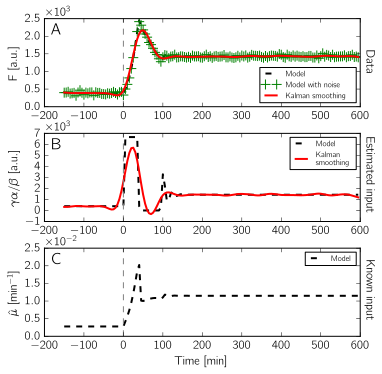
\includegraphics[scale=1]{./Fig/synthetic_upshift}
\caption{
\textbf{Performance of the Kalman smoothing procedure on synthetic data simulating an acetate-glucose upshift.}
\textit{(A)}~Synthetic data simulating an upshift from acetate to glucose, with and without additive white noise, as well as the results obtained by Kalman smoothing.
The synthetic data were generated by simulating the model presented in Eqs~\ref{eq:pdef}-\ref{eq:rdef} with the on-off regulatory strategy (Eq.~\ref{eq:stratswitch} and Fig.~\ref{fig:onoffresults}).
The model parameters used for the simulation are $e_{M,\texttt{Ace}} = 0.18$~h\textsuperscript{-1}, $e_{M,\texttt{Glu}} = 0.9$~h\textsuperscript{-1}, $k_R = 3.6$~h\textsuperscript{-1}, $\beta = 0.003$~L~g\textsuperscript{-1}, $K_R = 1$~g~L\textsuperscript{-1}.
The predicted $r(t)$ profile was multiplied by a factor $\gamma = 0.02$~RFU~L~g\textsuperscript{-1} in order to obtain the corresponding fluorescence intensity profile $F$ (dashed black curve).
The noise level was estimated from the data (\ref{S7_Text}) and added to $F$.
The choice of the parameters of the Kalman smoothing procedure is discussed in the Material and Methods~\ref{sec:meth_kalman}.
\textit{(B)}~Estimation of the resource allocation profile $\gamma \alpha / \beta$ based on the data in \textit{(A)}.
Following Chapter~\ref{chap:theory}, $\alpha (t)$ displays a bang-bang-singular profile during the upshift (dashed black curve).
While the Kalman smoother is not able to capture the discontinuous variations in $\gamma \alpha / \beta$, it qualitatively reproduces the input quite well (red solid curve).
\textit{(C)}~The predicted growth rate during the upshift experiment.
This information is used as an input in the smoothing procedure, since it is supposed to have been independently estimated from the measurements $\left\{L(t_0), ..., L(t_{N-1}) \right\}$.
}
\label{fig:synthetic_upshift}
\end{figure}

The results of the reconstruction of the resource allocation profile $u = \gamma \alpha (\cdot) / \beta$ are presented in Fig.~\ref{fig:gene_activity}.
Within the interval between -150 and 0 min, resource allocation remains more or less stable, as expected for steady-state growth on acetate.
On the contrary, the reconstructed resource allocation profile seems particularly unstable at the beginning and the end of the experiment.
While oscillations do occur after the upshift, these need to be taken with much care.
The problem of reconstructing an on-off strategy is more challenging than we initially thought, for the simple reason that the expected signal is similar to the kind of artifacts a poorly calibrated regularization method would generate.
Data about the pre-upshift and post-upshift steady state are crucial for the calibration of the method and, as explained in Section~\ref{sec:data_acquisition}, the experiment had to be interrupted before a steady state on glucose was attained.
We extensively discuss this and other problems in Section~\ref{sec:chap3_discussion} and give directions for future improvements.

\begin{figure}[p]
\centering
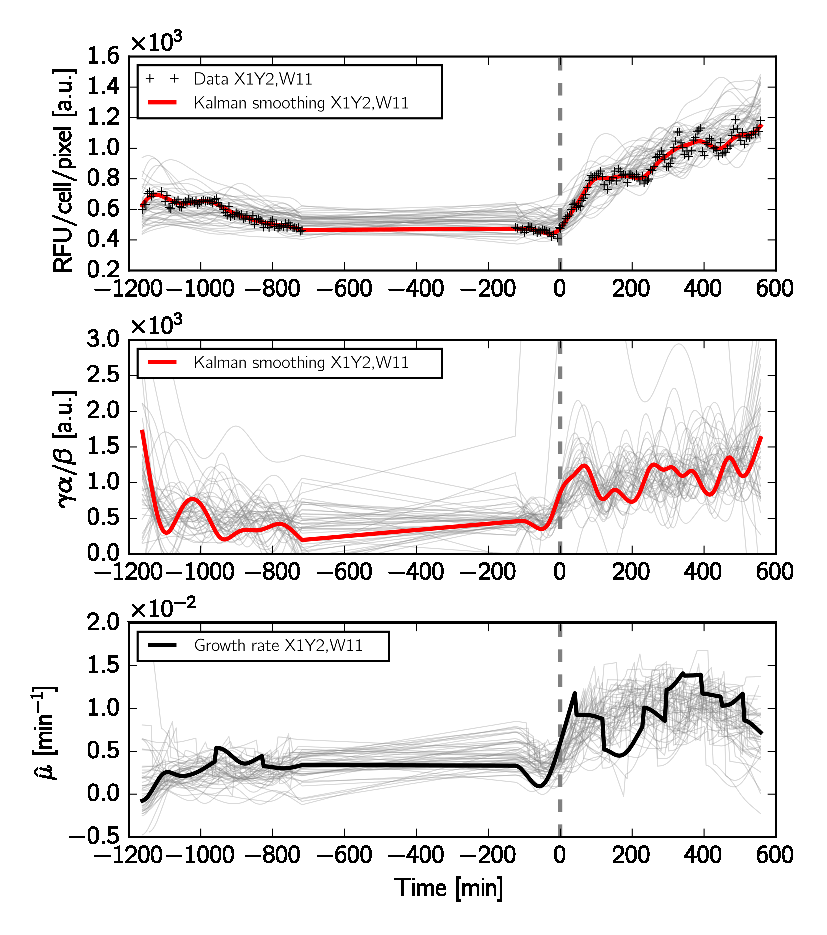
\includegraphics[scale=1]{./Fig/gene_activity}
\caption{
\textbf{Estimation of the resource allocation profile using Kalman smoothing based on the fluorescence density measurements and the estimated growth rates from Fig.~\ref{fig:growth_rate_estimation}.}
\textit{(A-B)} Gray lines represent the estimation of the fluorescence density (RFU/pixel) $F(\cdot)$ (in A) and the resource allocation profile $\gamma \alpha / \beta$ (in B) by the Kalman smoothing procedure for the 45 normal cells.
The solid red curves highlight the result for one particular cell, , located at the bottom of the well labelled "X3Y2, W2", while black crosses in the top graph are the data points for this cell.
The vertical dashed lines represent the time of the upshift from growth on acetate to growth on glucose.
The prior values for the parameters of the smoothing algorithm are exactly the same as those used for Fig.~\ref{fig:synthetic_upshift} and are reported in the Material and Methods~\ref{sec:meth_kalman}.
}
\label{fig:gene_activity}
\end{figure}

Nevertheless, when not focusing on the individual cells but looking at the statistics of the entire data set, some interesting patterns emerge. 
Fig.~\ref{fig:gene_activity_median} shows the median of the time-varying growth rate and resource allocation profile as well as the 25\%-75\% interquartile range. 
The use of these statistics gives a more robust view on the population level of the response of the cells to a nutrient upshift. 
When changing the carbon source from acetate to glucose, the growth rate increases to a value of around 0.011 min$^{-1}$, consistent with growth rates reported in the literature for the \textit{E. coli} strain used here~\cite{volkmer_condition-dependent_2011,izard_synthetic_2015}, before decreasing when the first cells start to die (Fig.~\ref{fig:gene_activity_median}\textit{C}).
In addition, the data show one period of an oscillation in the first 3~h after the upshift, conserved in each of the 25\%, 50\% and 75\% quartiles (Fig.~\ref{fig:gene_activity_median}\textit{B}).
The heatmap in Fig.~\ref{fig:gene_activity_heatmap} reveals that almost all of the normal cells show this oscillatory feature.
Moreover, the first peak is seen to be even more pronounced on the level of the individual cells, reflecting the fact that in the different cells it occurs at different times after the upshift and is therefore dampened out at the population level.
While the results of the microfluidic experiment presented here do not allow to confirm the occurrence of an on-off strategy for resource allocation after a nutrient upshift, the preliminary data are encouraging and prompt further investigation.

\begin{figure}[p]
\centering
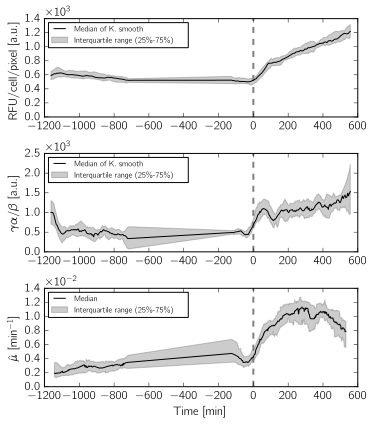
\includegraphics[scale=1]{./Fig/gene_activity_median}
\caption{
\textbf{Robust statistics for the estimation results presented in Fig.~\ref{fig:gene_activity}.}
Each graph shows the 25\% (lower gray curve), 50\% (solid black curve) and 75\% (upper gray curve) quartiles, computed at each time step for the signals reconstructed in Fig.~\ref{fig:gene_activity}.
The gray area represents the interquartile range.
Interestingly, while most oscillations in the resource allocation profile $\gamma \alpha (\cdot) / \beta$ cancel out at the population level, the first peak after the upshift is conserved.
}
\label{fig:gene_activity_median}
\end{figure}

\begin{figure}[tb]
\centering
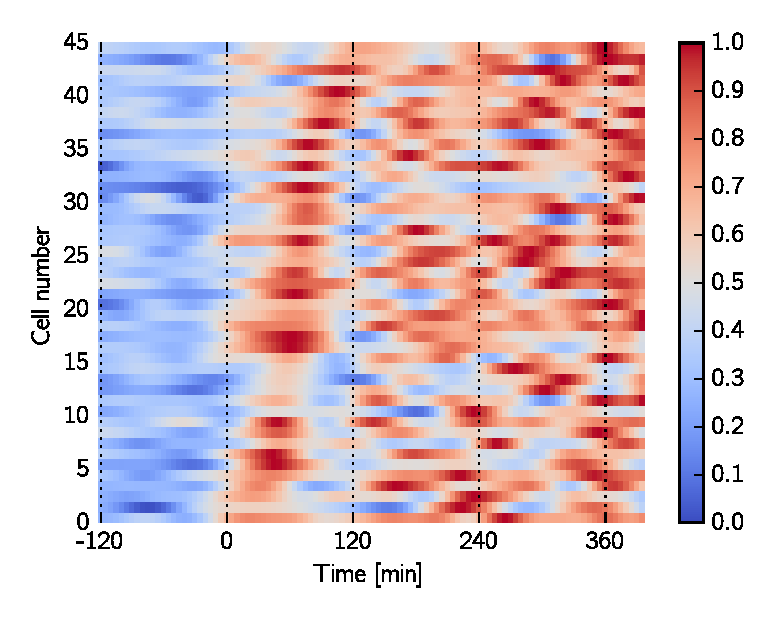
\includegraphics[scale=1]{./Fig/heatmap}
\caption{
\textbf{Global overview of all estimated resource allocation profiles presented in Fig.~\ref{fig:gene_activity}.}
The individual $\gamma \alpha (\cdot) / \beta$  curves have been normalized with respect to their maximum in the interval $[0, 400]$ and then ordered with respect to their maximum in the interval $[0, 120]$.
}
\label{fig:gene_activity_heatmap}
\end{figure}

\section{Discussion}
\label{sec:chap3_discussion}

As we showed in Chapter~\ref{chap:theory}, adopting a dynamical perspective might prove useful to unveil and understand the regulatory strategies employed by microorganisms.
The criterion of biomass maximization has allowed to account for steady-state empirical growth laws.
Interestingly, when the same criterion is applied to growth transitions, it predicts that microorganisms allocates their resources through bang-bang control of gene expression.
For the control of ribosome synthesis, the implementation of this optimal control scheme results in an on-off strategy, where a bacterial cell is either producing only ribosomes or not producing them at all during the adaptation to a new growth medium.
The ppGpp system, ubiquitous in bacteria and playing an important role in the control of ribosome synthesis in \textit{E. coli}, satisfies the requirements posed by the on-off strategy.
However, we currently lack experimental data to show that it actually functions in this manner, among other things because of the difficulties to produce well-controlled growth transitions on the single-cell level in the laboratory.
Can we set up appropriate experiments to measure the expression of ribosomes during a growth transitions?
Will the bacterial cells exhibit the on-off strategy that was shown to be close to optimal in Chapter~\ref{chap:theory}?

In this chapter, the above questions have been addressed by developing an experimental framework which allows the ribosome concentration to be quantified in individual \textit{E. coli} cells in real time.
Our main contribution consists in bringing together several experimental techniques developed in recent years.
First, inspired by the work of Bakshi \textit{et al.}~\cite{bakshi_superresolution_2012}, we constructed an \textit{E. coli} strain with fluorescent ribosomes.
In their paper, Bakshi \textit{et al} essentially used this fluorescent marker to localize ribosomes in the cytoplasm through superresolution microscopy.
While improving their design (Material and Methods~\ref{sec:methods_strain}), we used our strain for the purpose of quantifying ribosomal abundance in single cells.
Second, we employed the mother machine developed by Wang \textit{et al.}~\cite{wang_robust_2010}, originally developed to study long-term steady-state growth of \textit{E. coli}, to observe individual \textit{E. coli} cells growing in continuous culture by means of time-lapse fluorescence microscopy.
Here, the mother machine was used to establish well-controlled growth transitions, \textit{i.e.} from steady-state growth in minimal medium with acetate to steady-state growth in minimal medium with glucose.
By changing the medium source of the mother machine, we were able to observe how \textit{E. coli} cells adapt their growth rate and the expression of ribosomes.
Overall, through the combination of fluorescent labeling of a core component of the gene expression machinery and the use of a microfluidic device, we have opened the way to experimentally study growth laws in a dynamical context.

We applied this experimental setup to the reconstruction of the resources allocation strategy employed by \textit{E. coli} during a nutrient upshift, with the aim to observe the bang-bang profile predicted in Chapter~\ref{chap:theory}.
We developed a Kalman smoothing procedure adapted to our question and showed how it can be implemented to reconstruct the internal state of a cell from time-lapse microscopy images.
Similar to hidden Markov chains, Kalman filtering and smoothing are powerful techniques for the reconstruction of unobserved signals from noisy measurements, and have had numerous applications in a variety of domains, though less in biology than in other fields.
We showed in this chapter that the Bayesian framework of Kalman smoothing can be exploited for growth rate reconstruction from a probabilistic prior defining the relation between mother and daughter cells.
We also developed another variant of Kalman smoothing for the reconstruction of the resource allocation variable $\alpha (\cdot)$ that is at the heart of the models of Chapter~\ref{chap:theory}.
Our work on synthetic data showed that, despite the challenge posed by the reconstruction of a discontinuous signal, the algorithm was capable of recovering an oscillatory pattern close to the expected on-off profile.
Unfortunately, its application to the real data did not allow an unambiguous conclusion to be drawn: while oscillations do occur, and a first peak between 0 and 120 min after the upshift is visible in almost all of the cells, it turned out to be far from straightforward to distinguish a real oscillatory pattern from artifacts of the data analysis and signal reconstruction methods.
Below we propose several improvements that will be addressed in future work.

Several experimental problems complicated the analysis of the data.
Sufficiently long steady-state measurements before and after the transition of interest are needed to provide a reliable estimation of the intensity and the nature of the experimental noise.
They are also critical to calibrate the parameters of the regularization method used for signal reconstruction.
Despite what was initially planned, we did not completely reach a new steady state after the transition.
Several causes are to blame.
First, the random stall of the motorization along the Z-axis of the microscope, which does not allow overnight measurements and occurred during the slow growth on acetate in the presented experiment.
Second, the massive death of bacteria starting after the transition on glucose.
Future work will focus on solving these issues.

The death of bacteria is particularly worrying.
During the construction of this strain, most people in the lab experienced contamination by an aggressive bacteriophage.
Unfortunately, the strain used in this study was not spared, and our frozen stocks were later tested positive for phage-induced lysis.
Interestingly, the lysis seems to depend strongly on the environmental conditions.
To our disarray, the massive death observed in this experiment suggests that a strong environmental upshift could trigger the lytic cycle of the phage.
While impeding any possible long-term measurement, the death of the bacteria is not our only worry.
Phages are machines that are extremely well optimized to divert cell resources to their own end, especially the activity of the gene expression machinery.
That could dramatically perturb the cell regulation of resource allocation, and so the conclusions of this study.
For this reason, future work will start by the reconstruction of a clean phage-free strain from scratch.

It is also possible to optimize the image analysis techniques used in this study.
We segmented the images using the most powerful and ubiquitous segmentation algorithm available: the human brain.
In other words, we manually selected the pixels representing the poles of a single bacteria per well on the fluorescence images, and used this information to arbitrarily define a rectangle around the cell of interest.
While this is far from satisfying, it may turn out to be difficult to improve upon this, as it seems that the first rule of image analysis is that every application is more or less unique.
Every algorithm has to make assumptions about the object it is trying to recognize.
For imaging of microbial cells, it could be the curvature at the poles, the size of the pixels, the homogeneity of the background, the homogeneity of intracellular fluorescence, ...
While some parameters can be tweaked, some assumptions are always hard-coded in the algorithm and reflect the philosophy used to address the identification problem.
Since the preliminary analysis reported here was completed, we started a collaboration with the authors of FluoBacTracker~\cite{fluobactracker} that focuses on adapting their software to our setup in a near future.
It should provide a robust, automated way to identify and track the cells, enhancing the reproducibility of the analysis and increasing the number of cells available for computing population statistics.

The Kalman filtering algorithm that was later applied to these data can also be improved in many respects.
As described in the Results section, the algorithm is an instance of Bayesian inference and several parameters describing the expected input define a probabilistic prior.
In the work reported here, we chose these parameters through trial and error, or by calibrating the system on synthetic data whenever possible.
A better technique would be to choose these parameters by \textit{generalized cross-validation} (GCV)~\cite{golub_generalized_1979}, a procedure maximizing the predictive power of the reconstructed signal by reducing overfitting.
The use of GCV in our framework amounts to choosing the parameters of the Kalman smoother by optimizing predictions on a subset of the cells, then testing the performance on the remaining cells.
While the initial conditions did not seem to play a huge role in the final shape of the signal, the choice of the smoothing factor $\theta^2$ is critical and may strongly benefit from the proposed GCV extension.

The Kalman smoothing algorithm itself can also be further improved, notably by addressing the difficulty of estimating abrupt transitions.
As can be seen in Fig.~\ref{fig:synthetic_upshift}, the resource allocation profile $\gamma \alpha (\cdot) / \beta$ reconstructed from the synthetic data increases before the nutrient shift and this artifact also occurs when using the measured fluorescent densities (Fig.~\ref{fig:gene_activity_median}), the change in resource allocation preceding the nutrient upshift by several dozens of minutes.
While we know exactly when the change of medium occurs, this information is currently not used as a prior for the reconstruction.
The Kalman smoother can be improved by implementing time-varying parameters for the regularization method, so as to strongly penalize variations of the reconstructed signal at steady state and to release this constraint following the change in medium.

The improvements of the approach proposed in this section, which would help in reaching a conclusion about the existence of the on-off strategy, are not very complicated to realize.
Another improvement consists in taking into account the autofluorescence of the bacteria, which we assumed to be negligible, mostly because its proper estimation in a dynamical, single-cell context is complicated (Material and Methods~\ref{sec:cell_segmentation}).
A simple trick, however, could help in quantifying autofluorescence: mixing wild-type bacteria with bacteria having fluorescent ribosomes when loading the device.
This would allow some channels to be occupied by wild-type cells, in addition to the  channels in which the strain of interest is growing, and thus obtain a reliable estimation of the level of autofluorescence of the cells.
Notice though that the propertion between the two types of bacteria need to be carefully adjusted in order to preserve enough cells for the estimation of the resource allocation profile. 

%[I WOULD SKIP THIS FINAL PARAGRAPH OR REDUCE IT TO ONE PHRASE AND ADD IT TO THE DISCUSSION IN THE PARARAPH STARTING WITH "The Kalman smoothing algorithm..."]
%Something is also displeasing in the current implement of the Kalman smoothing method.
%As described in the main text, the Kalman smoothing procedure not only use previous measuments to estimate the state of the system, but also the next available measurements.
%This is a feature we totally lose in the estimation of the growth rate, because the discontinuities introduced by the cell divisions impede a global analysis of the time series.
%We partially solved the issue by using information about the mother cell at the beginning of the growth rate reconstruction of the daughter cells, but we did not find a way to implement it backward.
%There is probably a better way to deal with cell division in the analysis of microscopy data, and we are actively working on the matter.

\section{Material and Methods}

\subsection{Bacterial strain construction}

\label{sec:methods_strain}

In order to quantify the concentration of ribosomes in the cell in
real time, we constructed a strain  containing a translational fusion
of \textit{gfp\_mut2}~\cite{zaslaver_comprehensive_2006} to the
C-terminus of \textit{rpsB}, the gene coding for the ribosome subunit
S2. The design was inspired by the work of Bakshi \textit{et al}.,
who used a similar construction to measure the spatial distribution
of ribosomes in living \textit{E.~coli}~cells \cite{bakshi_superresolution_2012}.
However, contrary to Bakshi \textit{et al.}, and in order not to create
any interference with normal gene expression in the modified cells,
we decided to keep the intergenic region between \textit{rpsB} and
the downstream gene, \textit{tsf}, unchanged. Since the transcription
factor \textit{tsf} is under the control of the same promoter as \textit{rpsB},
leaving a selection marker downstream of \textit{rpsB} would interfere
with the proper expression of \textit{tsf}. Our strategy comprises
two steps: (i)~creation of the translational fusion by selecting
an antibiotic resistance marker and (ii)~removal of the selection
marker. The strategy is outlined in Figure~\ref{fig:Cloning}.

\begin{figure}[p]
\centering
\includegraphics[scale=1]{./Fig/meth_cloning}
\caption{
\textbf{Construction of the gfp-tagged ribosome subunit.}
The translational fusion of \textit{gfp\_mut2} with \textit{rpsB}
was constructed on the chromosome of \textit{E.~coli} (top line)
by homologous recombination of \textit{gfp\_mut2} followed by a selection
``cassette'' (second line). A small linker was inserted between
\textit{rpsB} and \textit{gfp\_mut2} in order to minimize interference
of the fluorescent protein with ribosome functioning. The selection
cassette consists of a positive selection marker, the gene coding
for the resistance to the antibiotic kanamycine, and a negative selection
marker, the gene coding for the toxin CcdB. The latter is transcribed
from the $p_{BAD}$ promoter, which is only activated in the presence
of arabinose in the culture medium. Homologous recombination is indicated
by the grey shaded lines. The resulting recombination product (third
line) contains the desired fusion protein followed by the selection
cassette on the chromosome of the bacterium. A second homologous recombination,
using an oligonucleotide complementary to the end of \textit{gfp\_mut2}
and the beginning the original region downstream of \textit{rpsB}
removes the selection cassette. The resulting strain (line four) carries
the translational fusion of \textit{gfp\_mut2} to \textit{rpsB} without
any other modification of the chromosome.}
\label{fig:Cloning}
\end{figure}

The DNA fragment containing the selection cassette was amplified using
two long primers annealing, respectively, downstream of \textit{rpsB} (starting just after
the STOP codon), and to the end of \textit{gfp\_mut2}.
The selection cassette contains an antibiotic resistance gene, kanamycin
(positive selection), and a gene coding for the CcdB toxin under the
control of the \textit{p\textsubscript{BAD}} promoter (negative selection
in presence of arabinose). This cassette is referred below as \textit{kan-p\textsubscript{BAD}-ccdB}.

Another DNA fragment containing \textit{gfp\_mut2}~\cite{zaslaver_comprehensive_2006}
without the ATG start codon was amplified using long primers annealing,
respectively, to the C-terminus of \textit{rpsB}
(just before the STOP codon), and the end of the \textit{kan-p\textsubscript{BAD}-ccdB}
cassette. The first primer also contained a 18-bp (base pair) linker,
inserting the same six amino-acids that Bakshi \textit{et al.} have used for their
construction ~\cite{bakshi_superresolution_2012}.

The two fragments, the \textit{gfp\_mut2} reporter including the linker
and the \textit{kan-p\textsubscript{BAD}-ccdB} cassette, were assembled
by Gibson assembly~\cite{gibson_enzymatic_2009} using a commercial
Gibson Assembly mix (New England Biolabs). A final product of 2683
bp was obtained: 
\begin{itemize}
\item {*}(50 bp) the C-terminus of \textit{rpsB} without the STOP codon 
\item (18 bp) a linker
\item (714 bp) the \textit{gfpmut2} sequence without the initial ATG 
\item (1851 bp) the \textit{kan-p\textsubscript{BAD}-ccdB} cassette 
\item {*}(50 bp) the region directly after \textit{rpsB} in \textit{E.~coli} 
\end{itemize}
Regions labeled with {*} anneal to the \textit{E.~coli} chromosome.
The complete sequence of this fragment, as well as the sequences of
all the primers, are listed in \ref{S5_Text}.

This fragment was electroporated into the wildtype strain, BW25113,
containing the pSIM5 plasmid for lambda-red recombinaison~\cite{sharan_recombineering_2009}.
A kanamycin-resistant colony was selected on LA-glucose medium and
verified to show green fluorescence (485~nm excitation, 535~nm emission) in a microplate reader (Tecan Infinite 200 pro).
A 100-bp oligonucleotide, containing 50 bp of the end of \textit{gfp\_mut2}
and 50 bp of the region just downstream of \textit{rpsB} was electroporated
into this strain (sequence available in \ref{S5_Text}). The
homologous recombination removes the \textit{kan-p\textsubscript{BAD}-ccdB}
cassette. A colony was selected on an LA-arabinose plate. The clone
was tested for kanamycin-sensitivity and  green fluorescence. Finally,
the strain was grown overnight at 42$^{\circ}$C to get rid of the
pSIM5 plasmid, containing a temperature-sensitive origin of replication.
A chloramphenicol-sensitive colony was chosen and the region after
\textit{rpsB} was verified by sequencing (full sequence obtained available in \ref{S5_Text}).

In parallel, the same protocol was used to construct \textit{mCherry}
and \textit{cfp} variants of the same strain. However, only the \textit{gfp\_mut2}
and \textit{mCherry} versions were successfully obtained. The full
sequence of the final \textit{rpsB-mCherry} strain is available in \ref{S5_Text}.

The \textit{rpsB-gfp} and \textit{rpsB-mCherry} strains were
characterized on different media using a Tecan microplate reader (\ref{S6_Text}, in particular Fig.~\ref{fig:suppinfo_caract} for growth on glucose).
They possess a wild-type growth rate and sufficient fluorescence to
allow quantification. However, the \textit{rpsB-mCherry} strain exhibited
strange fluorescence dynamics, especially during growth transitions,
which made it unsuitable for our study. We therefore concentrated
our efforts on the \textit{rpsB-gfp} strain (see \ref{S6_Text} for more details).

\subsection{Growth conditions}

\label{sec:growth_condition}

All experiments were carried out in sterilized media. Sterilization
was performed by autoclaving for instruments and filtration for solutions
(0.2 $\mu$m). During cloning, bacteria were grown in 20-mL Erlenmeyer
flasks filled with LB or spread on Petri dishes with LA. In all the
experiments, we used M9 minimal medium supplemented with trace elements,
thiamine and a carbon source. The full recipe is reproduced below.
Numbers in squared brackets are characteristics of the stock solution.
All stock solutions were stored at room temperature, except for FeSO$_{4}$~{[}30
g.L\textsuperscript{-1}{]} and Thiamine~{[}10 g.L\textsuperscript{-1}{]},
which were stored respectively at -20$^{\circ}$C and 4$^{\circ}$C. 

\begin{center}
\begin{tabular}{|l r|}
  \hline
  \multicolumn{2}{|c|}{\textbf{M9 medium (100 mL)}}\\
  \hline
  CaCl2 [1 mol.L\textsuperscript{-1}] & 10 $\mu$l\\
  MgSO$_4$ [1 mol.L\textsuperscript{-1}] & 200 $\mu$l\\
   5x Salts & 20 mL \\
  Traces elements & 90 $\mu$l \\
  FeSO$_4$ [30 g.L\textsuperscript{-1}] & 10 $\mu$l \\
  Thiamine [10 g.L\textsuperscript{-1}] & 50 $\mu$l \\
  Carbon source & at will \\
  H$_2$0 [18.2 M$\Omega$.cm] & to 100 mL \\
  \hline
\end{tabular}
\begin{tabular}{|l r|}
  \hline
  \multicolumn{2}{|c|}{\textbf{Traces elements (0.9 mL)}}\\
  \hline
  H$_2$0 [18.2 M$\Omega$.cm] & 200$\mu$l\\
  Na$_2$EDTA 2H$_2$O [150 g.L\textsuperscript{-1}] & 100$\mu$l\\
  ZnSO$_4$ 7H$_2$O [45 g.L\textsuperscript{-1}] & 100$\mu$l\\
  CoCl$_2$ 6H$_2$O [3 g.L\textsuperscript{-1}] & 100$\mu$l\\
  MnCl$_2$ 4H$_2$O [10 g.L\textsuperscript{-1}] & 100$\mu$l\\
  H$_3$BO$_3$ [10 g.L\textsuperscript{-1}] & 100$\mu$l\\
  Na$_2$MoO$_4$ 2H$_2$O [4 g.L\textsuperscript{-1}] & 100$\mu$l\\
  CuSO$_4$ 5H$_2$O [3 g.L\textsuperscript{-1}] & 100$\mu$l\\
  \hline
\end{tabular}
\begin{tabular}{|l r|}
    \hline
  \multicolumn{2}{|c|}{\textbf{5x Salts (100 mL)}}\\
  \hline
  Na$_2$HPO$_4$2H$_2$0 & 4.25 g \\
  KH$_2$HPO$_4$ & 1.5 mg \\
  NaCl & 0.25 g\\
  NH$_4$Cl& 0.5 g\\
  H$_2$0 [18.2 M$\Omega$.cm] & to 100 mL \\
  \hline
\end{tabular}
\end{center}

A large quantity of M9 was prepared several days before the experiment,
and stored at 4$^{\circ}$C. It contained all the necessary components
except FeSO$_{4}$, thiamine, and carbon sources, which were added
just before inoculation of the pre-culture. Except where stated otherwise,
the growth temperature was 37$^{\circ}$C. M9 Acetate contains 0.2\%
acetate (in mass of C$_{2}$H$_{3}$O$_{2}$ per mass of solution),
and M9 Glucose contains 0.2\% glucose (in mass of D-(+)-Glucose per
mass of solution).

Four days before the measurements, the glycerol stock containing the
\textit{rpsB-gfp} strain was spread on a Petri dish of LA, and incubated
at 37$^{\circ}$C. On the following day, an isolated colony was
used to inoculate a cotton-plugged, sterile flask containing 20 mL
of M9 acetate (Fig.~\ref{fig:experiment_schema}). The time of inoculation
was calculated such that the culture obtains an OD of 0.3-0.4 OD at
the beginning of the experiment. This optical density corresponds
to a culture in mid-exponential growth phase.

At the day of the experiment, the pre-culture was concentrated by centrifugation
and re-suspended in 5 mL of M9 acetate, supplemented with 50~mg.mL\textsuperscript{-1}
BSA (passivation buffer) for injection into the microfluidic device.
Channels were filled by diffusion until most of them contained cells
($\sim$1 hour). Data acquisition started after a constant medium
flow was successfully obtained ($\sim$1 hour, depending on the quality
of the microfluidics device).

\subsection{Microfluidic device}

\label{sec:microflu}

In order to observe the bacteria over a long time, we used the so-called
mothermachine~\cite{wang_robust_2010}. It consists of a series of
wells (or channels), oriented at a 90$^{\circ}$ angle to a large,
central channel through which growth medium is passed at a constant
flow rate. The width of the wells, a little over a $\mu m$, constrains
the bacteria to grow ``in a line''. This design ensures that at
least one cell per well (the one at the bottom of the channel) remains
in the device during the entire experiment, while the others incrementally
escape into the central channel as divisions occur. For the fabrication
of the devices, we thoroughly followed the step described in the supporting
information of~\cite{wang_robust_2010}. We maintained a stock of
chemically treated devices at room temperature (day 2 in workflow
summary~\cite{wang_robust_2010}). The day of the experiment, a single
device was plasma cleaned, bond to a glass coverslip, and injected
with bacteria (see section above).

The device was connected using 0.023\textquotedbl{} inner diameter
polyethylene tubes to a waste and a sterile bottle containing 200
mL of growth medium, which was enough for several days of acquisition.
A microfluidic pump (Elvesys) containing an output flow sensor module
was plugged to the medium bottle and a pressure up to 2~bars was
applied to the bottle. The output flow was set to 50 $\mu$L.min$^{-1}$.

For imaging, the device was placed on a motorized inverted microscope
(Zeiss Axiovert 200M) with a phase contrast objective lens (Zeiss
PlanNeofluar, Ph3 100x/1.3), placed in a thermostated box at 37$^{\circ}$C.
In this setup, fluorescence illumination is provided by a mercury
lamp (Osram, 1xHBO 103X/2) and visualization is performed with narrow-bandpass
excitation and emission filters (Chroma, \#49002 ET-GFP and Chroma,
\#49005 TR/DsRED ET). The exposure time is externally controlled by
mechanical shutters (Uniblitz-VS35). Images were acquired with a 16-bit
gray level CCDcamera cooled to -80$^{\circ}$C (Roper Scientific,
Princeton Instruments PHOTOMAX 512) controlled by a custom-made software
using Visual Basic and the Type libraries of the Winview software
(Princeton Instruments). Every 5 minutes, autofocus was numerically
performed by maximizing the contrast of a region of interest, and
a series of acquisitions were made. A total of 6 fields, each containing
15 wells was observed during the entire experiment.

\subsection{Cell segmentation}

\label{sec:cell_segmentation}

The raw data from the camera are in the form of 512x512-pixel 16-bit
SPE images (proprietary format produced by the Princeton Instruments
camera). They were converted into 16-bit Tif images using the \textit{SPE}
plugin of ImageJ~\cite{goto_open_2005}. The rest of the analysis
was performed using Python 3.5.2. In particular, we used OpenCV~3.1.0-dev,
Scikit-Image~0.12.3, Numpy~1.11.2 to manipulate the images.

In order to correct for the drift of the device, we calculated
the offset between consecutive images of a given field using cross-correlation
in the Fourier space~\cite{guizar-sicairos_efficient_2008} (see
Scikit-Image documentation at \cite{skimage_cross-correlation}).
All images for a field were thereby aligned to the first acquisition
by a simple translation.

In order to simplify the image treatment, we extracted individual
wells from the images by a combination of manual pixel selection and
automatic segmentation. In particular, we selected the entrance of
the two wells at the border of the image, and used this information
along with the regularity of the microfluidic device to compute a
mask that allowed to extract each well into an image of size 100x21
pixels. These sub-images were labeled $\left\{ W0,W1,...,W14\right\} $
depending on the position of the well in the original image, from
left to right.

In this study, we performed a preliminary analysis of each well, focusing
on the cell at the bottom of the channel. For each image, we manually
selected the poles of the cell of interest. The distance between the
two selected pixels was directly used as the length $L$ of the bacterium
in pixels. The two selected positions were also used to compute a
rectangular 6-pixel-wide mask around the cell (see Fig.~\ref{fig:data_acquisition}).
We then computed the RFU/pixel in this cell mask by summing each pixel
and dividing by the mask size.

The camera noise and background were evaluated by taking a picture
with a closed shutter at the end of the experiment. Pixels in this
picture were found to be Gaussian distributed with a mean of 1101.0
and a standard deviation of 10.788. A correction for the camera background
was thus applied by removing 1101 from the computed RFU/pixel.

The autofluorescence of the bacteria and the background fluorescence
of the medium were supposed to be negligible and were thus not corrected.
As a control, the same device was used to image bacteria in stationary
phase that do not produce any fluorescent protein. They were indistinguishable
from the camera noise. Of course, using this control we can not affirm
that the autofluorescence is also negligible when the bacteria are
actively growing. Furthermore, the autofluorescence could change in
different media of interest, and may even be different in steady state
and during growth transitions. An independent estimate of the autofluorescence
is therefore difficult to obtain. In the section~\ref{sec:chap3_discussion},
we discuss possible improvements of the experimental setup that would
allow to dynamically co-estimate the autofluorescence with the ribosome
abundance in a single experiment.

\subsection{Kalman smoothing}

\label{sec:meth_kalman}

The data of the length and the RFU/pixel of each bacteria were analyzed
using Python~3.5.2. In particular, we manipulated the data using
Pandas~0.19.1, Pykalman~0.9.5 and the Curves submodule of Wellfare~0.1.1.

Historical details about the Kalman smoothing procedure are reported
in section~\ref{sec:res_kalman} of the main text. We used the Additive
Unscented Kalman Filter implementation of the Pykalman python module.
This class is reported to be more stable and computationally efficient
with non-linear problems containing additive noise.

As described in section~\ref{sec:res_kalman}, the reconstruction
of the growth rate was done on continuous portions of the length,
\textit{i.e.} between cell divisions. The full problem, as described
in Eq.~\ref{eq:full_mu_prob}, is reproduced below for clarity: 
\begin{eqnarray*}
\dot{V_{\lambda}}(t) & = & \mu(t)\cdot V_{\lambda}(t),\\
\dot{\mu}(t) & = & v(t),\\
\dot{v}(t) & = & w(t),
\end{eqnarray*}
with the measurement model: 
\[
L(t_{k})=V_{\lambda}(t_{k})+\epsilon_{k},
\]
and the initial conditions
\[
V_\lambda (0) = V_{\lambda,0}, \;\;\;\; \mu (0) = \mu_0 , \;\;\;\; v(0) = v_0.
\]
The parameters used as priors for the reconstruction of $\mu$ are
described below. We used an observation variance of 9 pixels\textsuperscript{2}
for the length $L$. The transition variance $\theta^{2}$ (\textit{a.k.a.}
the smoothing factor for $\mu$) is fixed at $10^{-8}$~min\textsuperscript{-6}
for the entire time series. Inheritance between mother and daughter
cells is taken into account by systematically choosing an initial
mean for $\mu_0$ equal to the last estimated value for $\mu$, and for $V_{\gamma,0}$ to half the
last estimated value for $V_{\gamma}$ (as expected for a completely
symmetrical division). At the beginning of the experiment, when no
mother cells are available, these values were fixed to 15~pixels
for $V_{\gamma}$ and 0.004~min\textsuperscript{-1} for $\mu$.
The variances associated with these means are 16~pixels\textsuperscript{2}
and $10^{-4}$~min\textsuperscript{-2}, respectively, for $V_{\gamma,0}$
and $\mu_0$. The initial mean of $v$ is always taken as null, with
an initial variance of $10^{-8}$~min\textsuperscript{-6}. All the
cross-covariances are set to 0 because the system variables are independent
by construction.

For the reconstruction of gene activity, we had to cope with the large
gap in data acquisition between -720 and -150 min. Reconstruction
was then done independently on the continuous sections before and
after this gap. The full problem for the estimation of $u=\gamma\alpha/\beta$,
as described in Eq.~\ref{eq:full_u_prob}, is reproduced here for
clarity: 
\begin{eqnarray*}
\dot{r_{\gamma}}(t) & = & \hat{\mu}(t)\cdot u(t)-\hat{\mu}(t)\cdot r_{\gamma}(t),\\
\dot{u}(t) & = & v(t),\\
\dot{v}(t) & = & w(t),
\end{eqnarray*}
with the measurement model 
\[
F(t_{k})=r_{\gamma}(t_{k})+\eta_{k},
\]
and the initial conditions
\[
r_\gamma (0) = r_{\gamma,0}, \;\;\;\; u (0) = u_0 , \;\;\;\; v(0) = v_0,
\]
where $\hat{\mu}$ is the estimate of $\mu$ above. In both case,
we used as prior an observation variance of 800.4 RFU\textsuperscript{2}
for $F$. The transition variance $\theta^{2}$ (\textit{a.k.a.} the
smoothing factor for $\gamma\alpha/\beta$) is fixed at $10^{2}$~RFU\textsuperscript{2}.min\textsuperscript{-4}.
The initial state means used are 600~RFU for $r_{\gamma,0}$ and 1000~RFU
for $u_0$. The variances associated with these means
are purposely large and fixed at 10\textsuperscript{6}~RFU\textsuperscript{2}
for $r_{\gamma,0}$ and $u_0$. The initial mean for $v_0$
is always taken as null, with an initial variance of $10^{-8}$~RFU.min\textsuperscript{-2},
imposing a null second derivative for the reconstructed signal $\gamma\alpha/\beta$.
Here again, all the cross-covariances are set to 0.

All the parameters cited in this section were chosen through trial
and error, and are therefore certainly optimizable. Possible improvements
are discussed in Section~\ref{sec:chap3_discussion}.

\clearpage
\section{Supporting Information for Chapter~3}

\subsection{S5 Text -- DNA sequences used for the strain construction}
\manuallabel{S5_Text}{S5~Text}

\subsubsection{Exhaustive list of the primers used}

\paragraph{...for the \textit{gfp\_mut2} amplification.}

\begin{itemize}
\item[] 
\includegraphics[scale=1]{Fig/gfpmut2_L.png} \seqsplit{GTTCTCAGGATCTGGCTTCCCAGGCGGAAGAAAGCTTCGTAGAAGCTGAGCAGGAAAGGCGACAGGAGAGTAAAGGAGAAGAACTTTTCACTG}
(Length: 93)\\
\textit{The 50 first bp anneals with the C-terminus of \textit{rpsB} (just before the STOP codon).
The 18 next bp code for the linker (see Material and Methods~\ref{sec:methods_strain}).}
\item[] 
\includegraphics[scale=1]{Fig/gfpmut2_R.png} \seqsplit{TGATGTTCTGGGGAATATAATTATTTGTATAGTTCATCCATGCC} (Length: 44)\\
\textit{The 20 last bp anneals with the end of the \textit{kan-p\textsubscript{BAD}-ccdB} cassette.}
\end{itemize}

\paragraph{...for the \textit{mCherry} amplification}

\begin{itemize}
\item[] 
\includegraphics[scale=1]{Fig/mCherry_L.png} \seqsplit{GTTCTCAGGATCTGGCTTCCCAGGCGGAAGAAAGCTTCGTAGAAGCTGAGCAGGAAAGGCGACAGGAGACTAGCAAAAGATCCAAGGG}
(Length: 88)
\item[] 
\includegraphics[scale=1]{Fig/mCherry_R.png} \seqsplit{TGATGTTCTGGGGAATATAATTATTTGTACAGCTCATCCATG} (Length: 42)\\
\textit{Same design as for gfp\_mut2, except it amplifies mCherry.}
\end{itemize}

\paragraph{...for the cassette amplification}

\begin{itemize}
\item[] 
\includegraphics[scale=1]{Fig/cassette_L} \seqsplit{TGGATGAACTATACAAATAATTATATTCCCCAGAACATCAGG}
(Length: 42, used to assemble with gfp)\\
\textit{The 20 first bp anneals with the end of gfp\_mut2.}
\item[] 
\includegraphics[scale=1]{Fig/cassette_L} \seqsplit{TGGATGAGCTGTACAAATAATTATATTCCCCAGAACATCAG}
(Length: 41, used to assemble with mCherry)\\
\textit{The 20 first bp anneals with the end of mCherry.}
\item[] 
\includegraphics[scale=1]{Fig/cassette_R} \seqsplit{GAGCTTGCCGCCTTTCTGCAACTCGAACTATTTTGGGGGAGTTATCAAGCTTAGAAGAACTCGTCAAGAAGG}
(Length: 72, used for both)\\
\textit{The 50 last bp anneals downstream rpsB (just before the STOP codon).}
\end{itemize}


\paragraph{...for the whole insert amplification}

\begin{itemize}
\item[] 
\includegraphics[scale=1]{Fig/overlap_L} \seqsplit{GTTCTCAGGATCTGGCTTCCCAGG}
(Length: 24)
\item[] 
\includegraphics[scale=1]{Fig/overlap_R} \seqsplit{GAGCTTGCCGCCTTTCTGCA} (Length: 20)
\end{itemize}

\paragraph{...for the cassette elimination}

\begin{itemize}
\item[\textbf{\textit{rpsB-gfp}}] \seqsplit{TTGTAACAGCTGCTGGGATTACACATGGCATGGATGAACTATACAAATAAGCTTGATAACTCCCCCAAAATAGTTCGAGTTGCAGAAAGGCGGCAAGCTC}
(Length: 100)
\item[\textbf{\textit{rpsB-mCherry}}] \seqsplit{GCGCGGAGGGTCGTCATTCTACCGGTGGCATGGATGAGCTGTACAAATAAGCTTGATAACTCCCCCAAAATAGTTCGAGTTGCAGAAAGGCGGCAAGCTC}
(Length: 100)
\end{itemize}


\paragraph{...for the sequencing of the final strain}

\begin{itemize}
\item[] 
\includegraphics[scale=1]{Fig/sequencing_L} \seqsplit{CGTCTGAAAGACCTGGAAAC}
(Length: 20)
\item[] 
\includegraphics[scale=1]{Fig/sequencing_R} \seqsplit{AAACGTGTACTACCTGGTCTATAAGG} (Length: 26)
\end{itemize}

\subsubsection{Full annotated sequences of the inserts}

The following pages contain the full annotated sequences of the region downstream \textit{rpsB} after the insertion of \textit{gfp\_mut2-cassette} and \textit{mCherry-cassette}, respectively (third line in Fig.~\ref{fig:Cloning}).
The primers annealing positions are indicated using the same color code as in the description of the primers above.
The primers reported in the publication of Bakshi \textit{et al.}~\cite{bakshi_superresolution_2012} are indicated for information.

\includepdf[pages={1-7}]{./Fig/gfp_mut2-cassette-after-rpsB-E-coli-sequence.pdf}
\includepdf[pages={1-7}]{./Fig/mCherry-cassette-after-rpsB-E-coli-sequence.pdf}

\subsubsection{Sequencing of the final strains}

After the strains were made using the protocol described in Material and Methods~\ref{sec:methods_strain}, the downstream region of the \textit{rpsB} gene was amplified and sent for sequencing.
Alignments of the results showed they exhibit the expected sequences, except for a couple of single-base mutations.
The raw results of the sequencing are reproduced below.

\paragraph{Final sequences of the \textit{rpsB-gfp} strain (downstream region of \textit{rpsB})}

\begin{small}
\begin{itemize}
\item[] 
\includegraphics[scale=1]{Fig/sequencing_L} \seqsplit{AGAAAGAAGCGCTGTATGCGCACTCGTGAGCTGGAGAAACTGGAAAACAGCCTGGGCGGTATCAAAGACATGGGCGGTCTGCCGGACGCTCTGTTTGTAATCGATGCTGACCACGAACACATTGCTATCAAAGAAGCAAACAACCTGGGTATTCCGGTATTTGCTATCGTTGATACCAACTCTGATCCGGACGGTGTTGACTTCGTTATCCCGGGTAACGACGACGCAATCCGTGCTGTGACCCTGTACCTGGGCGCTGTTGCTGCAACCGTACGTGAAGGCCGTTCTCAGGATCTGGCTTCCCAGGCGGAAGAAAGCTTCGTAGAAGCTGAGCAGGAAAGGCGACAGGAGCGTAAAGGAGAAGAACTTTTCACTGGAGTTGTTCCAATTCTTGTTGAATTAGATGGTGATGTTAATGGGCACAAATTTTCTGTCAGTGGAGAGGGTGAAGGTGATGCAACATA}
\item[] 
\includegraphics[scale=1]{Fig/sequencing_R} \seqsplit{CGCCGCAGATGCGTTATCTTCGCTCGCTCATCCCGGTCACTTACTGATGTAAGCTCCCGGGAATTCTCGAGCTTGCCGCCTTTCTGCAACTCGAACTATTTTGGGGGAGTTATCAAGCTTATTTGTATAGTTCATCCATGCCATGTGTAATCCCAGCAGCTGTTACAAACTCAAGAAGGACCATGTGGTCTCTCTTTTCGTTGGGATCTTTCGAAAGGGCAGATTGTGTGGACAGGTAATGGTTGTCTGGTAAAAGGACAGGGCCATCGCCAATTGGAGTATTTTGTTGATAATGGTCTGCTAGTTGAACGCTTCCATCTTCAATGTTGTGTCTAATTTTGAAGTTAACTTTGATTCCATTCTTTTGTTTGTCTGCCATGATGTATACATTGTGTGAGTTATAGTTGTATTCCAATTTGTGTCCAAGAATGTTTCCATCTTCTTTAAAATCAATACCTTTTAACTCGATTCTATTAACAAGGGTATCACCTTCAAACTTGACTTCAGCACGTGTCTTGTAGTTCCCGTCATCTTTGAAAAATATAGTTCTTTCCTGTACATAAACCTTCGGGCATGGCACTCTTGAAAAAGTCATGCTGTTTCATATGATCTGGGTATCTCGCAAAGCATTGAAGACCATACGCGAAAAGTAGTGACAAGTGTTGGCCATGGAACAGGTAGTTTTCCAGTAGTGCAAATAAATTTAAGGGTAAAGTTTTCCGTATGTTGCATCACCTTCACCCTCTCCACTGACAGAAAAATTTGTGCCCATTTAACATCACCATCTAATTCAACAAGAATTGGAAACAACTCCAGTGAAAGT} 
\end{itemize}
\end{small}

\newpage
\paragraph{Final sequences of the \textit{rpsB-mCherry} strain (downstream region of \textit{rpsB})}

\begin{small}
\begin{itemize}
\item[] 
\includegraphics[scale=1]{Fig/sequencing_L}
\seqsplit{TTTCGACAGCTGACCAAGAAGAAGCGCTGATGCGCACTCGTGAGCTGGAGAAACTGGAAA
ACAGCCTGGGCGGTATCAAAGACATGGGCGGTCTGCCGGACGCTCTGTTTGTAATCGATG
CTGACCACGAACACATTGCTATCAAAGAAGCAAACAACCTGGGTATTCCGGTATTTGCTA
TCGTTGATACCAACTCTGATCCGGACGGTGTTGACTTCGTTATCCCGGGTAACGACGACG
CAATCCGTGCTGTGACCCTGTACCTGGGCGCTGTTGCTGCAACCGTACGTGAAGGCCGTT
CTCAGGATCTGGCTTCCCAGGCGGAAGAAAGCTTCGTAGAAGCTGAGCAGGAAAGGCGAC
AGGAGACTAGCAAAAGATCCAAGGGCGAGGAGGATAACATGGCTATCATTAAAGAGTTCA
TGCGCTTCAAAGTTCACATGGAGGGTTCTGTTAACGGTCACGAGTTCGAGATCGAAGGCG
AAGGCGAGGGCCGTCCGTATGAAGGCACCCAGACCGCCAAACTGAAAGTGACTAAAGGCG
GCCCGCTGCCTTTTGCGTGGGACATCCTGAGCCCGCAATTTATGTACGGTTCTAAAGCGT
ATGTTAAACACCCAGCGGATATCCCGGACTATCTGAAGCTGTCTTTTCCGGAAGGTTTCA
AGTGGGAACGCGTAATGAATTTTGAAGATGGTGGTGTCGTGACCGTCACTCAGGACTCCT
CCCTGCAAGATGGCGAGTTCATCTATAAAGTTAAACTGCGTGGTACTAATTTTCCATCTG
ATGGCCCGGTGATGCAGAAAAAGACGATGGGTTGGGAGGCGTCTAGCGAACGCATGTATC
CGGAAGATGGTGCGCTGAAAGGCGAAATTAAACAGCGCCTGAAACTGAAAGATGGCGG}
\item[] 
\includegraphics[scale=1]{Fig/sequencing_R}
\seqsplit{TTCGCGCCGCAGATGCGTTATCTTCGCTCGCTCATCCCGGTCACTTACTGATGTAAGCTC
CCGGGAATTCTCGAGCTTGCCGCCTTTCTGCAACTCGAACTATTTTGGGGGAGTTATCAA
GCTTATTTGTACAGCTCATCCATGCCACCGGTAGAATGACGACCCTCCGCGCGCTCATAT
TGCTCTACGATCGTATAATCTTCATTATGAGAGGTGATGTCCAGTTTAATATTCACATTG
TACGCGCCAGGCAGCTGCACAGGTTTCTTGGCTTTGTACGTGGTTTTCACTTCAGCGTCA
TAATGGCCGCCATCTTTCAGTTTCAGGCGCTGTTTAATTTCGCCTTTCAGCGCACCATCT
TCCGGATACATGCGTTCGCTAGACGCCTCCCAACCCATCGTCTTTTTCTGCATCACCGGG
CCATCAGATGGAAAATTAGTACCACGCAGTTTAACTTTATAGATGAACTCGCCATCTTGC
AGGGAGGAGTCCTGAGTGACGGTCACGACACCACCATCTTCAAAATTCATTACGCGTTCC
CACTTGAAACCTTCCGGAAAAGACAGCTTCAGATAGTCCGGGATATCCGCTGGGTGTTTA
ACATACGCTTTAGAACCGTACATAAATTGCGGGCTCAGGATGTCCCACGCAAAAGGCAGC
GGGCCGCCTTTAGTCACTTTCAGTTTGGCGGTCTGGGTGCCTTCATACGGACGGCCCTCG
CCTTCGCCTTCGATCTCGAACTCGTGACCGTTAACAGAACCCTCCATGTGAACTTTGAAG
CGCATGAACTCTTTAATGATAGCCATGTTATCCTCCTCGCCCTTGGAT} 
\end{itemize}
\end{small}

\clearpage
\subsection{S6 Text -- Strain validation in batch growing conditions}
\manuallabel{S6_Text}{S6~Text}

The \textit{rpsB-gfp} and \textit{rpsB-mCherry} strains were characterized on different media using a Tecan microplate reader.
Strains were grown in M9 minimal medium at 37$^\circ$C in 96-well microplates.
The absorbance and fluorescence were measured approximately every minute for up to 24~h.
In a single experiment, this allowed to generate up to 96 growth curves like the one schematized in Fig.~\ref{fig:growth_curve}.

In Fig.~\ref{fig:suppinfo_caract}, we show growth curves obtained on M9 supplemented with 0.2\% glucose.
As for the construction of Bakshi \textit{et al.}~\cite{bakshi_superresolution_2012}, our strains possess a wild-type growth rate (Fig.~\ref{fig:suppinfo_caract}A), indicating that the gfp-tagging or mCherry-tagging of the ribosomal S2 subunit does not impede the functioning of the ribosome.
It is known that \textit{E.~coli} cultures exhibit a high autofluorescence in the GFP bandwidth~\cite{mihalcescu_green_2015}, but the fluorescence of the \textit{rpsB-gfp} strain is at least 4-time higher than the \textit{wild-type} (Fig.~\ref{fig:suppinfo_caract}B).
Contrary to green autofluorescence, red autofluorescence of \textit{E.~coli} cultures is very low (Fig.~\ref{fig:suppinfo_caract}B) so the corrected signal level for mCherry is even more stronger.
Overall, both strains possess enough fluorescence to allow quantification at the population level, all the more so at the cell level because most part of the autofluorescence is concentrated in the medium outside the cell~\cite{mihalcescu_green_2015}.

In Fig.~\ref{fig:suppinfo_caract}C, we display the ratio between the (corrected) fluorescence of the strain and the absorbance (corrected means that we substracted the autofluorescence of the wild-type strain).
As a first approximation, this ratio can be used as a proxy for the fluorescence concentration in the cells, therefore for the ribosome concentration.
The instability at the beginning of the experiment (before 400~min) is characteristic of the difficulty to obtain robust estimations when the absorbance of the culture is low~\cite{zulkower_robust_2015}.
The RFU/Abs ratio is stable in the interval [400,600]~min for both \textit{rpsB-gfp} and \textit{rpsB-mCherry} strains, and can be interpreted as exponential steady-state growth.
Note that this short time interval (a couple of generations) of readability before approaching the stationary phase is one of the main problem preventing the use of batch conditions to obtain robust data about growth transitions.
Indeed, most of our attempt to perform robust growth transitions in this region were unsuccessful.

Results for \textit{rpsB-gfp} and \textit{rpsB-mCherry} start to differ when glucose is exhausted and the cells enter stationary phase.
As would be expected, the fluorescence of the \textit{rpsB-gfp} strain starts to slowly decrease as GFP proteins are degraded or photobleached.
On the contrary, the fluorescence of the \textit{rpsB-mCherry} strain quickly triples when entering stationary phase, at a rate that is way higher than the physical limit imposed by the protein synthesis rate~\cite{scott_interdependence_2010}.

\begin{figure}[p]
\centering
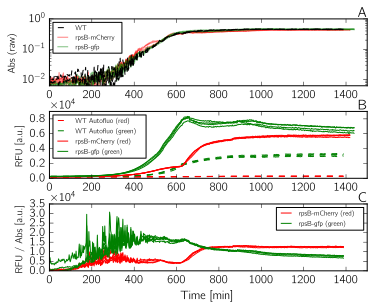
\includegraphics[scale=1]{./Fig/suppinfo_caract}
\caption{
\textbf{Growth curves in M9~0.2\% glucose for the \textit{rpsB-gfp} and \textit{rpsB-mCherry} strains.}
Growth and measurements were performed in a 96-well microplate placed in a Tecan infinite 200 pro reader thermostated at 37$^\circ$C.
We monitored 4 wells inoculated with the WT strain, the \textit{rpsB-gfp} strain, and the \textit{rpsB-mCherry} strain, for a total of 12 wells each containing 150~$\mu$L of growth medium.
Curves were shifted in time to correct for pipetting variability in the inoculation process (-50 min for WT, and -20 min for \textit{rpsB-mCherry}).
\textit{(A)}~The light absorbance as measured by the Tecan microplate reader, corrected for background by removing M9 absorbance.
The superposition of the curves indicates similar growth rates between the WT and the modified strains.
\textit{(B)}~The fluorescence measured in the wells, expressed in Relative Fluorescence Units (RFU).
Green fluorescence (485~nm excitation, 535~nm emission) is measured for the WT (dashed lines) and the \textit{rpsB-gfp} (solid lines) strains.
Red fluorescence (560~nm excitation, 635~nm emission) is measured for the WT (dashed lines) and the \textit{rpsB-mCherry} (solid lines) strains.
As can be seen, fluorescence levels of the modified strains are far above the autofluorescence measured on the WT strain.
\textit{(C)}~The ratio of fluorescence over absorbance, a proxy for the fluorescence concentration in the cells.
Autofluorescence background was corrected by removing the autofluorescence measured on the WT wells.
We observe a strange increase in fluorescence concentration for the \textit{rpsB-mCherry} strain at stationary phase, something does not occur on the \textit{rpsB-gfp} strain.
Before each measurement cycle, the following procedure was applied: shaking (Orbital 6mm) for 30~s, shaking (Linear 6mm) for 30~s, waiting for 5~s.
}
\label{fig:suppinfo_caract}
\end{figure}

In order to explain these strange dynamics, we set-up an experiment to evaluate the degradation and maturation rates of GFP and mCherry in our strains.
The procedure was to instantly stop all protein synthesis in mid-exponential phase using an antibiotic, then to observe the evolution of the fluorescence in a condition with no synthesis of new reporter proteins.
The estimation was performed using the following model:
\begin{eqnarray}
\frac{dP_m}{dt} &=& K \cdot P - (\mu+D) \cdot P_m, \\
\frac{dP}{dt} &=& f(t) - (\mu+D+K) P,
\end{eqnarray}
where $P_m$ is the concentration of mature (fluorescent) proteins, $P$ is the concentration of immature (non-fluorescent) proteins, $K$ is the maturation rate, $D$ is the degradation rate (assumed identical for mature and immature proteins), $f(t)$ the protein synthesis rate, and $\mu$ the growth rate.
By stopping all protein synthesis in the bacteria, we obtain $f(t) = \mu = 0$, hence the model becomes:
\begin{eqnarray}
\frac{dP_m}{dt} &=& K \cdot P - D \cdot P_m, \\
\frac{dP}{dt} &=& - (D+K) P.
\end{eqnarray}
This system of differential equations can be analytically solved into:
\[
P_m(t) = \left(P_m(0) + P(0) \left( 1 - e^{-Kt} \right) \right) e^{-Dt}
\]
with $P_m(0)$ and $P(0)$ the initial concentrations of mature proteins and immature proteins, respectively.
By dividing by $P_m(0)$ and taking the log of both sides, we can rewrite it as
\begin{equation}
\log \frac{P_m(t)}{P_m(0)} = - Dt + \log \left(1 + \frac{P(0)}{P_m(0)} \left( 1 - e^{-Kt} \right) \right).
\label{eq:matur_deg}
\end{equation}
Since growth is stopped, the bacterial volume is constant and then $\frac{P_m(t)}{P_m(0)}$ can be easily measured by directly taking the fluorescence normalized by its initial value, while the maturation rate $K$, the degradation rate $D$, and the initial fraction of immature proteins $\frac{P(0)}{P_m(0)}$ are free parameters that can be fitted on fluorescence time series.
The curves used for the estimation are represented in Fig.~\ref{fig:suppinfo_matur} and the results are reported in Tab.~\ref{tab:suppinfo_matur}.
As expected, both reporter proteins are stable and exhibit a long half-life in exponential phase (>24~h).
The maturation rate of GFP was too fast to obtain numerical value.
However, the maturation rate of mCherry is rather slow, with a half-maturation time in the order of 30~min (time needed to mature 50\% of a pool of mCherry).
Even though degradation and maturation rate can be slightly different in stationary phase, the estimated value are not sufficient to explain the rapid increase in fluorescence observed in Fig.~\ref{fig:suppinfo_caract}.

\begin{figure}[tb]
\centering
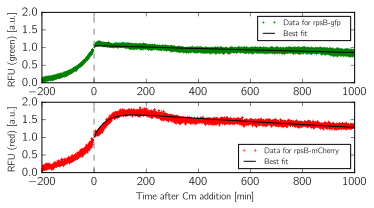
\includegraphics[scale=1]{./Fig/suppinfo_matur}
\caption{
\textbf{Estimation of the maturation and degradation rates of the reporter proteins in the \textit{rpsB-gfp} and \textit{rpsB-mCherry} strains.}
The strains were grown in the same condition as in Fig.~\ref{fig:suppinfo_caract}, except that a massive dose of Chloramphenicol was added in mid-exponential phase ($t=0$, vertical dashed grey line).
The fluorescence was normalized by the value at $t=0$ and the degradation and maturation rates were estimated by using the model in Eq.~\ref{eq:matur_deg}.
Parameters of the best fit (solid black line) are reported in Tab.~\ref{tab:suppinfo_matur}.
Data are the result of the aggregation of 9 and 8 independent growth curves for \textit{rpsB-gfp} and \textit{rpsB-mCherry}, respectively.
}
\label{fig:suppinfo_matur}
\end{figure}

\begin{table}[tb]
\begin{tabular}{|c|c|c|}
\hline
& \textbf{GFP mut2} & \textbf{mCherry}\\
\hline
\textbf{$P(0) / P_m(0)$} & 0.05635 $\pm$ 0.001202  & 0.7349 $\pm$ 0.0027362\\
\hline
\textbf{$D$~[min\textsuperscript{-1}]} & 0.0002064 $\pm$ 2.066e-06 & 0.0003027 $\pm$ 2.645e-06\\
\hline
\textbf{half-life~[min]}& 3325 - 3392 & 2269 - 2309\\
\hline
\textbf{$K$~[min\textsuperscript{-1}]} & $\emptyset$ & 0.02254 $\pm$ 0.0003\\
\hline
\textbf{half-maturation~[min]} & $\emptyset$  &  30.27 - 31.16\\
\hline
\end{tabular}
\caption{\textbf{Fitted parameters for the degradation and maturation of GFP mut2 and mCherry, according to the model in Eq.~\ref{eq:matur_deg} and data in Fig.~\ref{fig:suppinfo_matur}}}
\label{tab:suppinfo_matur}
\end{table}

The fluorescence of GFP and mCherry is known to be affected by intracellular physiological changes like pH or pO\textsubscript{2}~\cite{doherty_stage-specific_2010}.
In particular, mCherry has been reported to be extremely sensible to the presence of oxygen for its maturation~\cite{doherty_stage-specific_2010}.
We however reproduced the following results in conditions were the oxygen is not limiting.
In particular, the abrupt increase of mCherry fluorescence is conserved when the stationary phase is attained at low bacterial density, in a larger volume (20-mL flask), and on several type of carbon sources (acetate, xylose, glycerol, maltose).
We have so far no explanation for this strange dynamic, and therefore concentrated our effort on the \textit{rpsB-gfp} strain in the microfluidic experiments.

\clearpage
\subsection{S7 Text -- Noise estimation in the microscopy experiment}
\manuallabel{S7_Text}{S7~Text}

We estimated the noise in the RFU/pixel/cell measurements by using the data points just before the upshift (Fig.~\ref{fig:noise_poi}).
Since they have been growing for 20~h on acetate in the microfluidic device, bacteria are assumed in balanced growth in this region of $\sim$2~hours (roughly 23-24 points depending on the well of interest).
For this reason, ribosome concentration, and so fluorescence concentration, are expected constant.
Fig.~\ref{fig:noise_poi} shows the distribution of points in this region, that can be approximated by a Gaussian distribution, for a particular cell.

\begin{figure}[p]
\centering
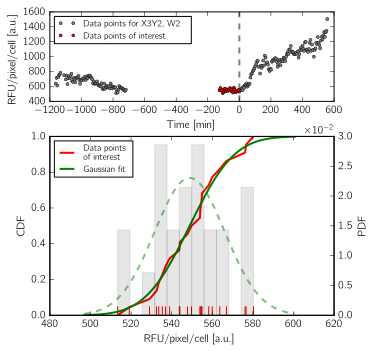
\includegraphics[scale=1]{./Fig/noise_poi}
\caption{
\textbf{Points of interest for the noise estimation.}\newline
\textit{(Top graph)} RFU/pixel/cell data points for the cell at the bottom of the well labeled X3Y2,W2.
Noise estimation was performed on the points just before the upshift (red points), were the bacteria is assumed to grow at steady state.
\textit{(Bottom graph)} Cumulative density function (CDF, in red) and probability density function (PDF, in gray) of the points highlighted in red on the top graph.
They are visually compared with CDF (solid green line) and PDF (dashed green line) of a Gaussian fit with mean 548.88 and standard deviation 17.316.
}
\label{fig:noise_poi}
\end{figure}

Interestingly, as can be seen in Fig.~\ref{fig:noise_distrib_mean_std}, the mean and standard deviation of the distribution vary from cell to cell in a slightly correlated manner (Pearson R\textsuperscript{2}: $0.3213$, p-value: $4.923\cdot10^{-5}$).
We did not investigate if this heterogeneity between cells is the result of true biological variations or a bias due to the microfluidic device.
By looking at the points of Fig.~\ref{fig:noise_distrib_mean_std}, there are however no strong correlation of the mean and standard deviation with the acquisition field (XY), or the position of the well on the image (W).

\begin{figure}[tb]
\centering
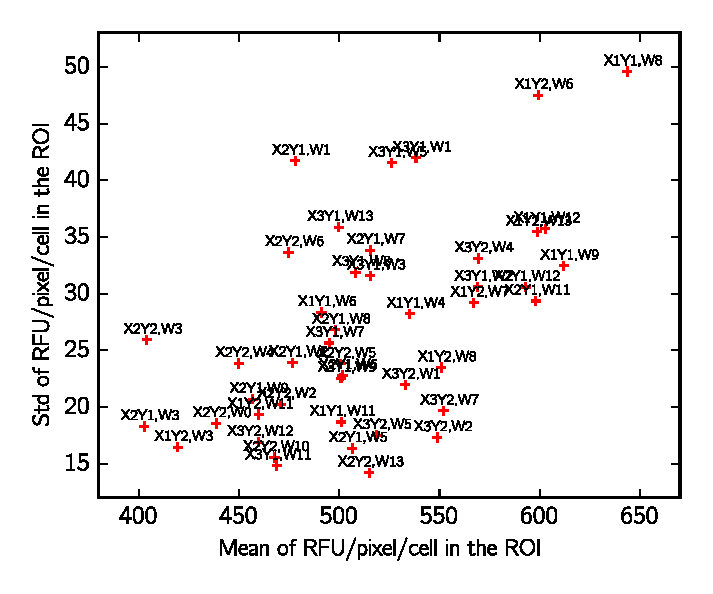
\includegraphics[scale=1]{./Fig/noise_distrib_mean_std}
\caption{
\textbf{Distribution of the means and standard deviations in the region of interest for the normal cells.}
The empirical mean and standard deviation were evaluated in the region before the upshift (red points on Fig.~\ref{fig:noise_poi}) for each of the 45 normal cells.
They appear to be slightly correlated (Pearson R\textsuperscript{2}: $0.3213$, p-value: $4.923\cdot10^{-5}$) which could indicate a multiplicative instead of an additive noise.
}
\label{fig:noise_distrib_mean_std}
\end{figure}

Noise characteristics were computed by normalizing and aggregating data for the 45 normal cells presented in Fig.~\ref{fig:noise_distrib_mean_std}.
Two scenarii were considered.
First, the noise model can be considered additive, which means we have the measurement model presented in Section~\ref{sec:estim_gr_ra}:
\begin{equation}
F(t_k) = \gamma r (t_k) + \eta_k,\\
\end{equation}
were $F(t_k)$ is the fluorescence measured at the time step $t_k$, $r (t_k)$ is the true ribosomal concentration at this time step, $\gamma$ is an unknown factor, and $\eta_k$ is the measurement noise.
In this scenario, for a time independent ribosome concentration $r$ (\textit{i.e.} at steady state), the ribosome concentration is equal to its mean on the interval of interest (noted $m_k(\cdot)$).
Given that
\begin{equation}
m_k (F) = m_k (\gamma r) + m_k(\eta_k) = \gamma m_k (r),\\
\end{equation}
the noise residues are given by
\begin{equation}
\eta_k = F(t_k) - m_k (F). \label{eq:noise_add}
\end{equation}
In other words, we can normalize the data points of each cell by removing their mean in order to aggregate the noise residues and get an estimation of the noise level (Fig.~\ref{fig:noise_estim_add_mul}, top panel).

Alternatively, the noise model can be considered multiplicative.
The noise model is than different than presented in Section~\ref{sec:estim_gr_ra}, and can be re-written:
\begin{equation}
F(t_k) = \gamma r (t_k) \cdot (1 + \lambda_k),
\end{equation}
were $\gamma r (t_k) \cdot \lambda_k$ is the measurement noise, proportional to the value measured.
In that scenario, with the same notations as above, the noise $\lambda_k$ is given by
\begin{equation}
\lambda_k = \frac{F(t_k)}{m_k (F)} - 1, \label{eq:noise_mul}
\end{equation}
which means we can normalize data points from different cells by dividing by the mean and removing 1 (Fig.~\ref{fig:noise_estim_add_mul}, bottom panel).

Both models were considered and are represented in Fig.~\ref{fig:noise_estim_add_mul}.
Despite the correlation identified in Fig.~\ref{fig:noise_distrib_mean_std}, the means of the residues in both models are very close to zero, and the distributions are well approximated by a Gaussian distribution.
For this reason, we decided in the main analysis to stick with an additive noise, the main reason being that the implementation used for the Kalman smoothing procedure are faster and more stable with an additive noise model.
We assumed an additive white Gaussian noise with mean 0 and standard deviation 28.29 for the simulation of the synthetic data and the signal reconstruction through the Kalman smoothing procedure.
As discussed in Section~\ref{sec:chap3_discussion}, the only way to decisively choose a noise model over the other would have been to obtain two different steady-state growths for each cell.
Unfortunately, the presented time series were not long enough to obtain a new steady state on glucose, something that will be corrected in future instances of the experiment.

\begin{figure}[p]
\centering
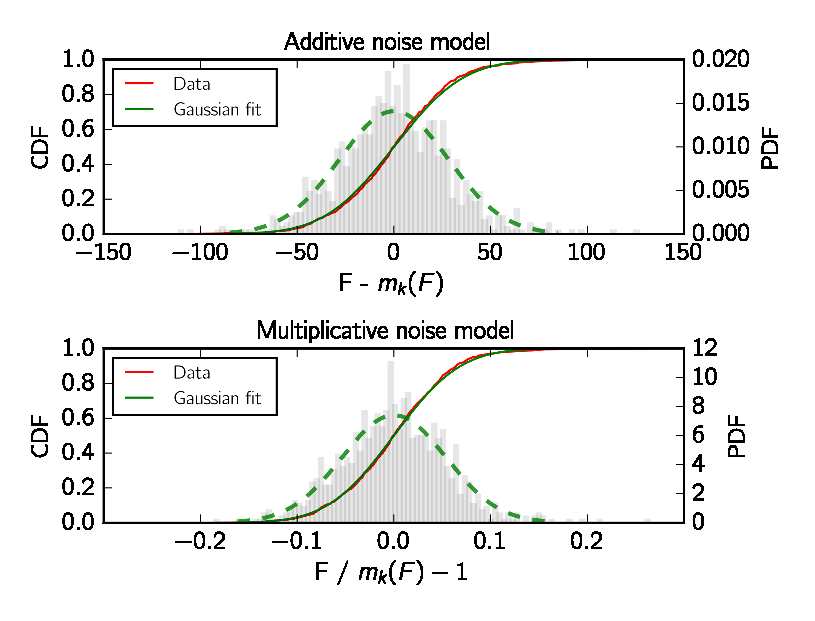
\includegraphics[scale=1]{./Fig/noise_estim_add_mul}
\caption{
\textbf{Distribution of the noise residues after normalization and aggregation for the 45 normal cells.}
Two noise models were considered for the normalization: either the temporal mean $m_k (\cdot)$ was removed from the measurements independently for each cell (additive noise model in Eq.~\ref{eq:noise_add}), or $1$ was removed from the ratio of the measurements with the temporal mean $m_k (\cdot)$ (multiplicative noise model in Eq.~\ref{eq:noise_mul}).
For the additive noise model, the fitted Gaussian distribution as a mean of $1.256\cdot 10^{-15}$ and a standard deviation of 28.29.
For the multiplicative noise model, the fitted Gaussian distribution as a mean of $2.666\cdot 10^{-18}$ and a standard deviation of 0.05383.
}
\label{fig:noise_estim_add_mul}
\end{figure}

\clearpage
\subsection{S8 Text -- Examples of complete analysis for 5 normal cells}
\manuallabel{S8_Text}{S8~Text}

In order to get a more visual idea of the results of the analysis, we display below the complete signal reconstructions for 5 cells.
In Figs~\ref{fig:cell1}-\ref{fig:cell5}, the image on the left is the last image analyzed for the corresponding well.
The bacteria either at the top or the bottom (depending on the orientation in the device) was manually segmented by selecting two pixels at the poles on the fluorescence images (red cross).
A 6-pixel-wide rectangular mask was computed for each image, resulting in the masked image on the right.
In each of the graphs, the black and green points represent data points, while the red solid lines are the results of the signal reconstruction \textit{via} the Kalman smoothing procedure.
The parameters of the Kalman smoothing are described in Material and Methods~\ref{sec:meth_kalman} and Figs~\ref{fig:growth_rate_estimation} and \ref{fig:gene_activity}.
Specific comments on each cell are given in the caption of Figs~\ref{fig:cell1}-\ref{fig:cell5}.

\begin{figure}[p]
\centering
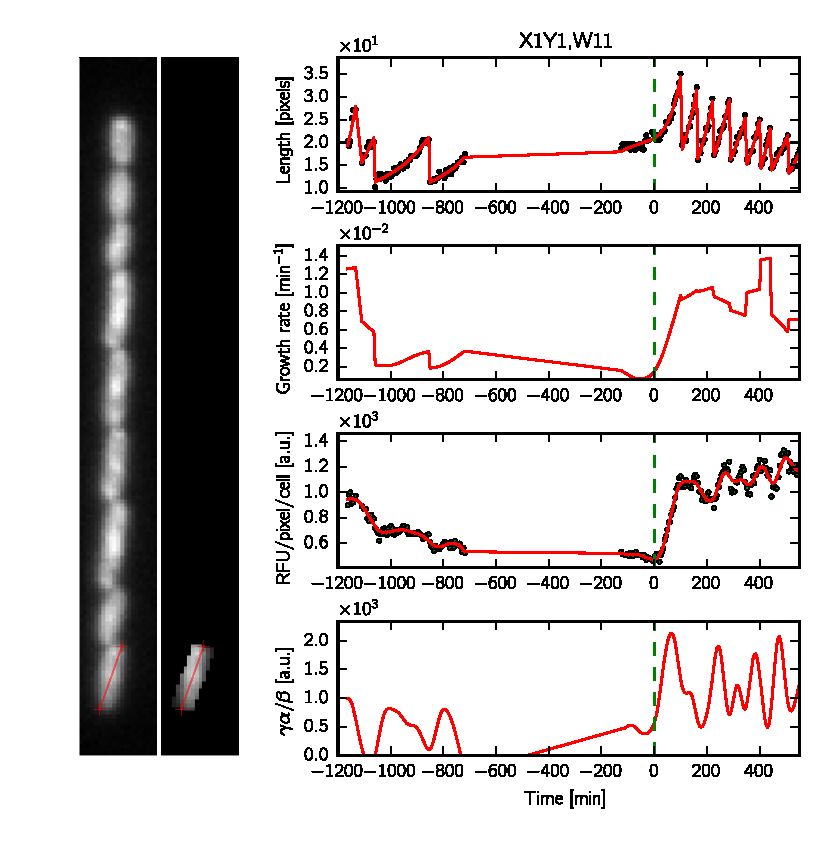
\includegraphics[scale=1]{./Fig/cell1}
\caption{
\textbf{Complete analysis for the cell located at the bottom of the well labelled "X1Y1, W11".}
(Figure description available in the introduction of \ref{S8_Text}.)\newline
Growth rate and resource allocation are particularly unstable at the beginning of the experiment, but seems to have stabilized before the upshift.
Oscillations in the RFU/pixel/cell signal are clearly visible, and result in oscillations in the resource allocation signal reconstruction.
}
\label{fig:cell1}
\end{figure}

\begin{figure}[p]
\centering
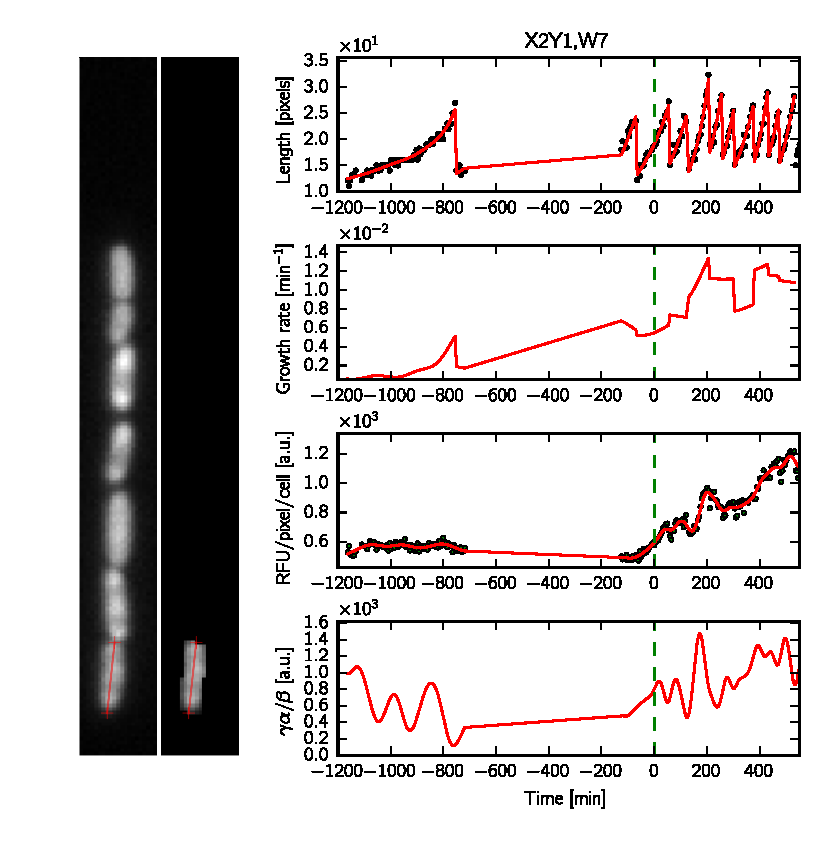
\includegraphics[scale=1]{./Fig/cell2}
\caption{
\textbf{Complete analysis for the cell located at the bottom of the well labelled "X2Y1, W7".}
(Figure description available in the introduction of \ref{S8_Text}.)\newline
Here, the resource allocation is unstable at the beginning of the experiment despite the apparent regularity of the RFU/pixel/cell.
This could indicate a smoothing factor that is too low for this particular cell.
}
\label{fig:cell2}
\end{figure}

\begin{figure}[p]
\centering
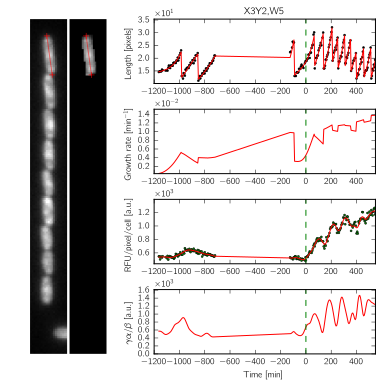
\includegraphics[scale=1]{./Fig/cell3}
\caption{
\textbf{Complete analysis for the cell located at the bottom of the well labelled "X3Y2, W5".}
(Figure description available in the introduction of \ref{S8_Text}.)\newline
We see for this cell that the reconstruction of the growth rate on the acetate medium (before 0) is affected by the huge gap in the acquisition, the increase before -150~min clearly being an artifact.
However, because the Kalman smoothing procedure we used allows for flexibility between the mother and the daughter cells, we quickly recover a more realistic growth rate before the upshift.
Despite an instability at the beginning of the experiment, the resource allocation reconstruction exhibits a remarkable stability during growth on the acetate medium, followed by oscillations after the upshift on glucose (also visible directly on the RFU/pixel/cell data).
}
\label{fig:cell3}
\end{figure}

\begin{figure}[p]
\centering
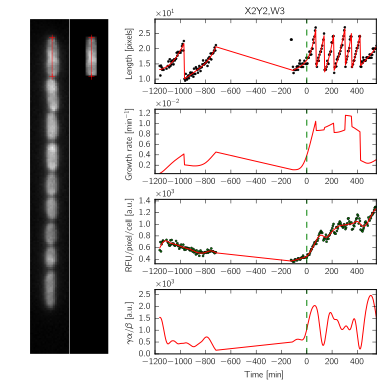
\includegraphics[scale=1]{./Fig/cell4}
\caption{
\textbf{Complete analysis for the cell located at the bottom of the well labelled "X2Y2, W3".}
(Figure description available in the introduction of \ref{S8_Text}.)\newline
The reconstruction on this cell is a good instance of what was expected: the growth rate is stable on acetate, than quickly increases after the upshift on glucose.
The resource allocation is stable on acetate (indicating a steady state) than starts to oscillate after the upshift on glucose, even though the smoothing factor seems a little too high for this particular cell (some oscillations are poorly predicted after the upshift, in particular in the interval [200,400]~min).
}
\label{fig:cell4}
\end{figure}

\begin{figure}[p]
\centering
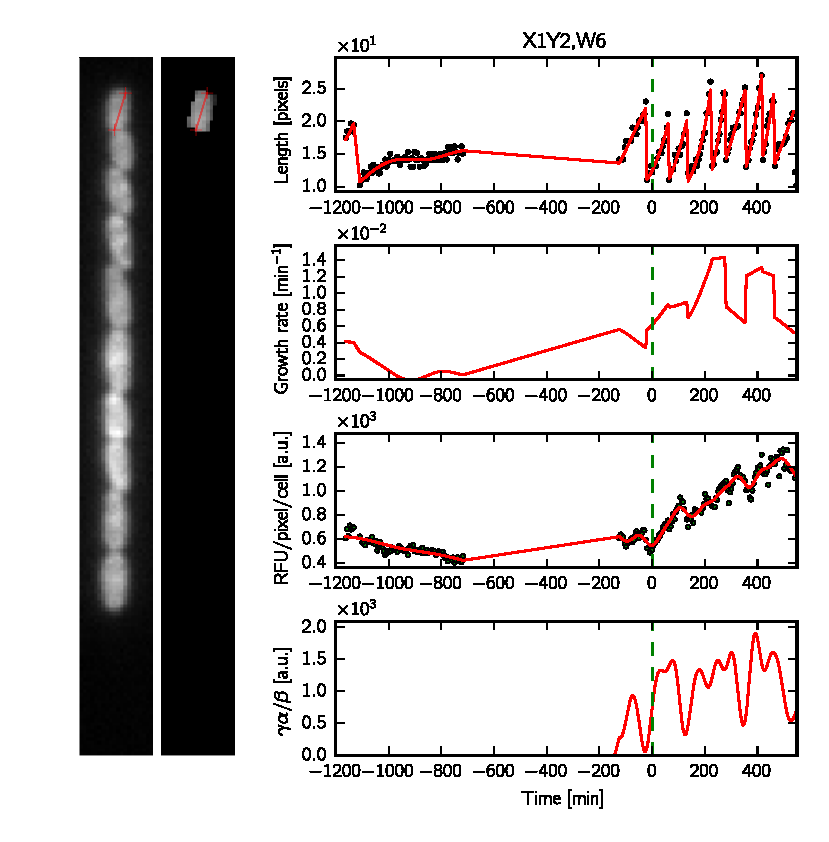
\includegraphics[scale=1]{./Fig/cell5}
\caption{
\textbf{Complete analysis for the cell located at the bottom of the well labelled "X1Y2, W6".}
(Figure description available in the introduction of \ref{S8_Text}.)\newline
The results on this cell are particularly terrible: we do not seem to get a good steady state on acetate since the reconstructed resource allocation appears either negative or oscillating before the upshift.
It is thus impossible to conclude if the oscillations observed after the upshift are real or due to overfitting.
This cell highlights why robust steady states before and after the transition are important to conclude on the signal reconstruction.
}
\label{fig:cell5}
\end{figure}

\clearpage
\subsection{S2 Figure -- Cell categories identified in the microscopy analysis}
\manuallabel{S2_Figure}{S2~Fig}

\begin{figure}[!h]
\centering
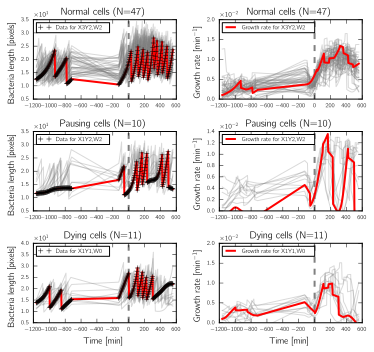
\includegraphics[scale=1]{./Fig/subcat_cells}
\caption{
\textbf{Cell categories identified in the microscopy analysis.}
As stated in Section~\ref{sec:estim_gr_ra}, the reconstruction of the growth rate for the 68 available cells motivated their classification in three categories: dying cells stop growing (lowest graphs) , pausing cells present growth rate oscillations (middle graph), and normal cells does not present any of the above (highest graph).}
\label{fig:subcat_cells}
\end{figure}

\clearpage
\subsection{S3 Figure -- Robust statistics for the cell categories}
\manuallabel{S3_Figure}{S3~Fig}

\begin{figure}[h]
\centering
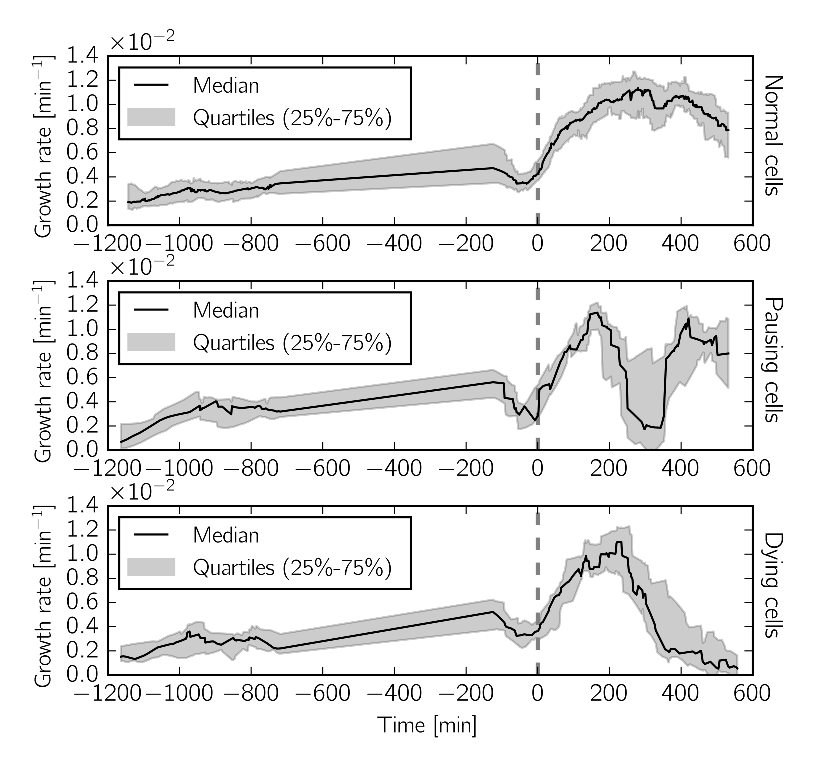
\includegraphics[scale=1]{./Fig/subcat_median}
\caption{
\textbf{Robust statistics for the cell categories identified in the microscopy analysis.}
Each graph shows the 25\% (lower gray curve), 50\% (solid black curve) and 75\% (upper gray curve) quartiles, computed at each time step for the growth rates presented in~\ref{S2_Figure}.
The gray area represents the interquartile range.
}
\label{fig:subcat_median}
\end{figure}